\documentclass[a4paper,12pt]{article}
\usepackage{silence}
\WarningFilter{latex}{Command \underline  has changed} % don't know where these come from
\WarningFilter{latex}{Command \underbar  has changed}
\usepackage[dvipsnames]{xcolor}
\usepackage[utf8]{inputenc}
\usepackage[T1]{fontenc}
\usepackage[parfill]{parskip}
\usepackage{mathtools}
\usepackage{enumitem}
\usepackage{csvsimple}
% \usepackage[perpage]{footmisc}
\usepackage{tabularx}
\usepackage[nottoc,numbib]{tocbibind}
\usepackage{algorithmicx}
\usepackage{algpseudocode}
\newcommand{\Continue}{\State\textbf{continue}}
\newcommand{\Yield}[1]{\State\textbf{yield} #1}
\usepackage{algorithm}
\usepackage{pdfpages}

\newif\iffast
% \fasttrue
\newcommand{\elnaturale}{\mathbb{N}}
\newcommand{\Oh}[1]{\mathcal{O} (#1)}
\usepackage{siunitx}
\sisetup{detect-all} % not math font or something

\iffast
\newcommand{\missingfigure}[1]{}
\newcommand{\todo}[1]{}
\usepackage{verbatim}
\newenvironment{tikzpicture}[1]{\comment}{\endcomment}
\else
% \usepackage{todonotes}
\usepackage{tikz}
\usetikzlibrary{arrows,positioning,calc,fit,arrows.meta,shadows}
\tikzset{big arrow/.style={-{Stealth[scale=1.4]}, shorten >=2pt}}
\tikzset{AST/.style = {
  minimum size=15pt,
  inner sep=0pt,
  every node/.style={circle, align=center},
  level distance=30pt,
}}
\usepackage{pgfplots}\pgfplotsset{compat=1.16}

\newcommand{\verticalline}[2]{\draw[#1]
($(current bounding box.north west)!#2!(current bounding box.north east)$)
--
($(current bounding box.south west)!#2!(current bounding box.south east)$)}
\fi

\usepackage{listings}
\usepackage{courier} % \texttt{...} gives thinner text and /\ displays OK

\newcommand\mznfont{\fontfamily{pcr}\selectfont}

\lstdefinestyle{mzn}{
  basicstyle=\mznfont,
  commentstyle=\color[rgb]{0.9,0.1,0.1},
  keywordstyle=\color[rgb]{0,0.5,0},
  keywordstyle=[2]\color{blue},
  stringstyle=\color{orange},
  tabsize=2,
  frame=none,
  % identifierstyle = \it,
  numbers=left,
  stepnumber=1,
  numberstyle=\tiny,
  numbersep=5pt,
  xleftmargin=0pt, % numbers will be in the margins!
  columns=fixed, % same width for all characters
  % columns=flexible,
  % columns=fullflexible,
  aboveskip={0pt},
  belowskip={0pt},
  showstringspaces=false,
  mathescape=true,
  breaklines=true,
  % prebreak=\raisebox{0ex}[0ex][0ex]{\ensuremath{\space\red{\swarrow}}},%\hookrightarrow
  % postbreak=\raisebox{0ex}[0ex][0ex]{\ensuremath{\textcolor{black}{\hookrightarrow\space}}},%\hookrightarrow
  % NOTE: beamer doesn't like color in postbreak.
  % https://tex.stackexchange.com/questions/586477/missing-number-treated-as-zero-within-beamer-and-lstcustom
  postbreak=\raisebox{0ex}[0ex][0ex]{\ensuremath{\hookrightarrow\space}},%\hookrightarrow
  breakatwhitespace=true,
  breakindent=0pt, % was: 20pt
  escapeinside={{<@}{@>}}
}

\lstdefinestyle{nonumbers} {
  numbers=none,
  xleftmargin=0pt,
}

\lstdefinelanguage{Mzn}
{
  morekeywords={
  %
  array, par, var, opt, constraint, solve, satisfy, minimize,
  maximize, output, include, let, in, set, of, if, then, else, endif,
  ann, annotation, bool, enum, float, int, string, where, function,
  predicate, true, false, not, assert, trace,
  % ???:
  any, list, op, record, test, tuple, type
  %
  },
  %
  keywords=[2]{
  %
  forall, sliding_sum, symmetry_breaking_constraint,
  implied_constraint, redundant_constraint, all_different,
  alldifferent, alldifferent_except_0, alldiff, element, circuit,
  subcircuit, dpath, card, bool2int, inter, count, regular, table, xor,
  exists, xorall, iffall, clause, intersect, diff, symdiff, subset,
  superset, concat, join, length, int_lt_reif, int_lin_eq_reif,
  bool_imply, array_bool_or, all_different_int, int_ne, at_least,
  at_most, exactly, count_eq, count_leq, count_geq, count_gt, nvalue,
  bin_packing, bin_packing_capa, bin_packing_load, diffn,
  global_cardinality, global_cardinality_closed, distribute,
  global_cardinality_low_up, global_cardinality_low_up_closed,
  inverse, cumulative, disjunctive, decreasing, increasing,
  strictly_decreasing, strictly_increasing, sort,
  arg_sort, value_precede, value_precede_chain, lex_less, lex_lesseq,
  lex_greater, lex_greatereq, lex2, strict_lex2, int_lin_eq, all_equal,
  bool_lin_eq, knapsack, partition_set, member, reverse, among, in_set,
  % from ???:
  abort, abs, acosh, array_intersect, array_union, array1d, array2d,
  array3d, array4d, array5d, array6d, asin, atan, bool2int, card,
  ceil, concat, cos, cosh, dom, dom_array, dom_size, fix, exp, floor,
  index_set, index_set_1of2, index_set_2of2, index_set_1of3,
  index_set_2of3, index_set_3of3, index_set_6of6, int2float, is_fixed,
  join, lb, lb_array, length, ln, log, log2, log10, min, max, pow,
  product, round, set2array, show, show_int, show_float, sin, sinh,
  sqrt, sum, tan, tanh, trace, ub, ub_array, xor, in, subset,
  superset, union, diff, symdiff, intersect, div, mod,
  % annotations:
  is_defined_var, output_var, var_is_introduced, defines_var,
  promise_total, bounds, domain, bool_search, int_search, seq_search,
  set_search, input_order, first_fail, anti_first_fail, smallest,
  largest, occurrence, most_constrained, max_regret, indomain_min,
  indomain_max, indomain_middle, indomain_median, indomain,
  indomain_random, indomain_split, indomain_reverse_split,
  indomain_interval, outdomain_max, outdomain_median, outdomain_min,
  outdomain_random, complete
  % 
  },
  sensitive=true,
  morecomment=[l]{\%},
  morestring=[b]",
  % morestring=[d]',
  moredelim=**[is][\color{Melon}]{@}{@},
}
%% Write "\begin{frame}[fragile]" for a slide using either of the
%% following two listing environments, which have unnumbered
%% respectively numbered lines:
\lstnewenvironment{mzn}[1][]{\lstset{language=Mzn,style=mzn,#1}}{}
\lstnewenvironment{mznno}[1][]{\lstset{language=Mzn,style=mzn,style=nonumbers,#1}}{}
\lstnewenvironment{mznnobreak}[1][]{\noindent\lstset{language=Mzn,style=mzn,style=nonumbers,#1}\minipage{\textwidth}}{\endminipage}
\BeforeBeginEnvironment{mznnobreak}{\par}
\AfterEndEnvironment{mznnobreak}{\par}

\lstnewenvironment{mznbreak}[1][]{\noindent\lstset{language=Mzn,style=mzn,#1}\minipage{\textwidth}}{\endminipage}
\BeforeBeginEnvironment{mznbreak}{\par}
\AfterEndEnvironment{mznbreak}{\par}
%% Inline a code snippet, without respectively with the comprehension bar (|):
\newcommand{\mzninline}[1]{\lstinline[{language=Mzn,style=mzn}]|#1|}
\newcommand{\mzninlinebar}[1]{\lstinline[{language=Mzn,style=mzn}]!#1!}

\newcommand{\mi}[1]{\mbox{\mzninline{#1}}}
\newcommand{\cpp}[1]{\mbox{\mznfont #1}}

\lstdefinestyle{diff}{
  morecomment=[f][\color{Green}]{+},
  morecomment=[f][\color{Red}]{-},
}
\lstnewenvironment{cppp}[1][]{\lstset{language={[11]C++},style=mzn,#1}}{}

\lstdefinestyle{floaty}{
  captionpos=b,
  frame=lines,
}

\usepackage{UppsalaExjobb}

\babelhyphenation[english]{Mini-Zinc}

% To get the same float style as the rest of the document
\newfloat{Listing}
\restylefloat{listing}

\newcommand{\leblanc}{\clearpage\thispagestyle{empty}\null\clearpage}
\newcommand{\ruleref}[1]{``\nameref{sec:rule:#1}'' (Section~\ref{sec:rule:#1})}

\begin{document}
% För att ställa in parametrar till IEEEtranS/IEEEtranSA behöver detta ligga här (före första \cite).
% Se se IEEEtran/bibtex/IEEEtran_bst_HOWTO.pdf, avsnitt VII, eller sista biten av IEEEtran/bibtex/IEEEexample.bib.
%%%% OBS: här ställer ni t.ex. in hur URLer ska beskrivas.
\bstctlcite{rapport:BSTcontrol}

\title{A Linter for Static Analysis of MiniZinc Models}
%\subtitle{beskrivande men gärna lockande}

\author{Erik Rimskog}

% Visa datum på svenska på förstasidan, även om ni skriver på engelska!
\date{\begin{otherlanguage}{swedish}
\today
\end{otherlanguage}}

\handledare{Pierre Flener}
\reviewer{Justin Pearson}
\examinator{Lars-Åke Nordén}
\seriesname{Examensarbete 30 hp}
\seriesnumber{UPTEC IT21~022}

% \maketitle
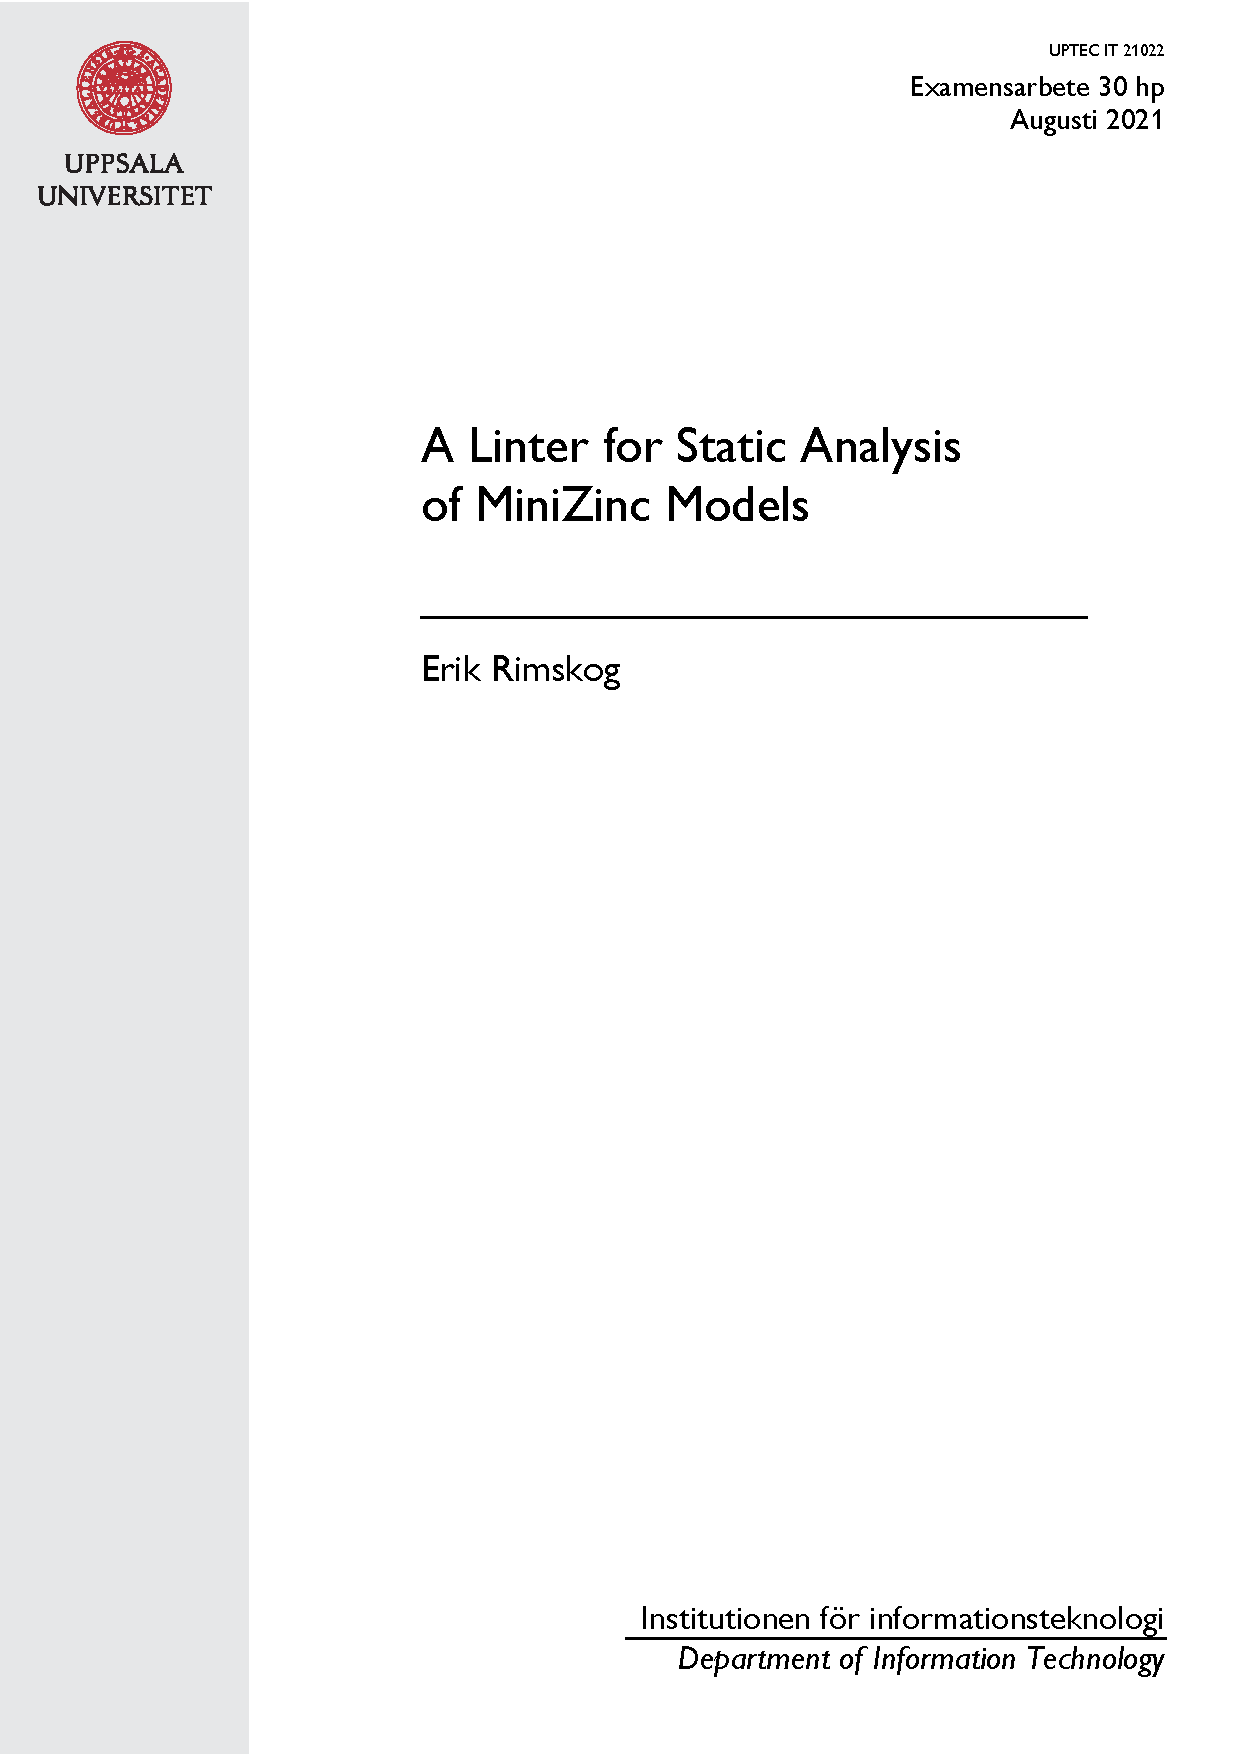
\includepdf[noautoscale=true]{Exjobbsframsida.pdf}

\leblanc

% Change to frontmatter style (e.g. roman page numbers)
\frontmatter

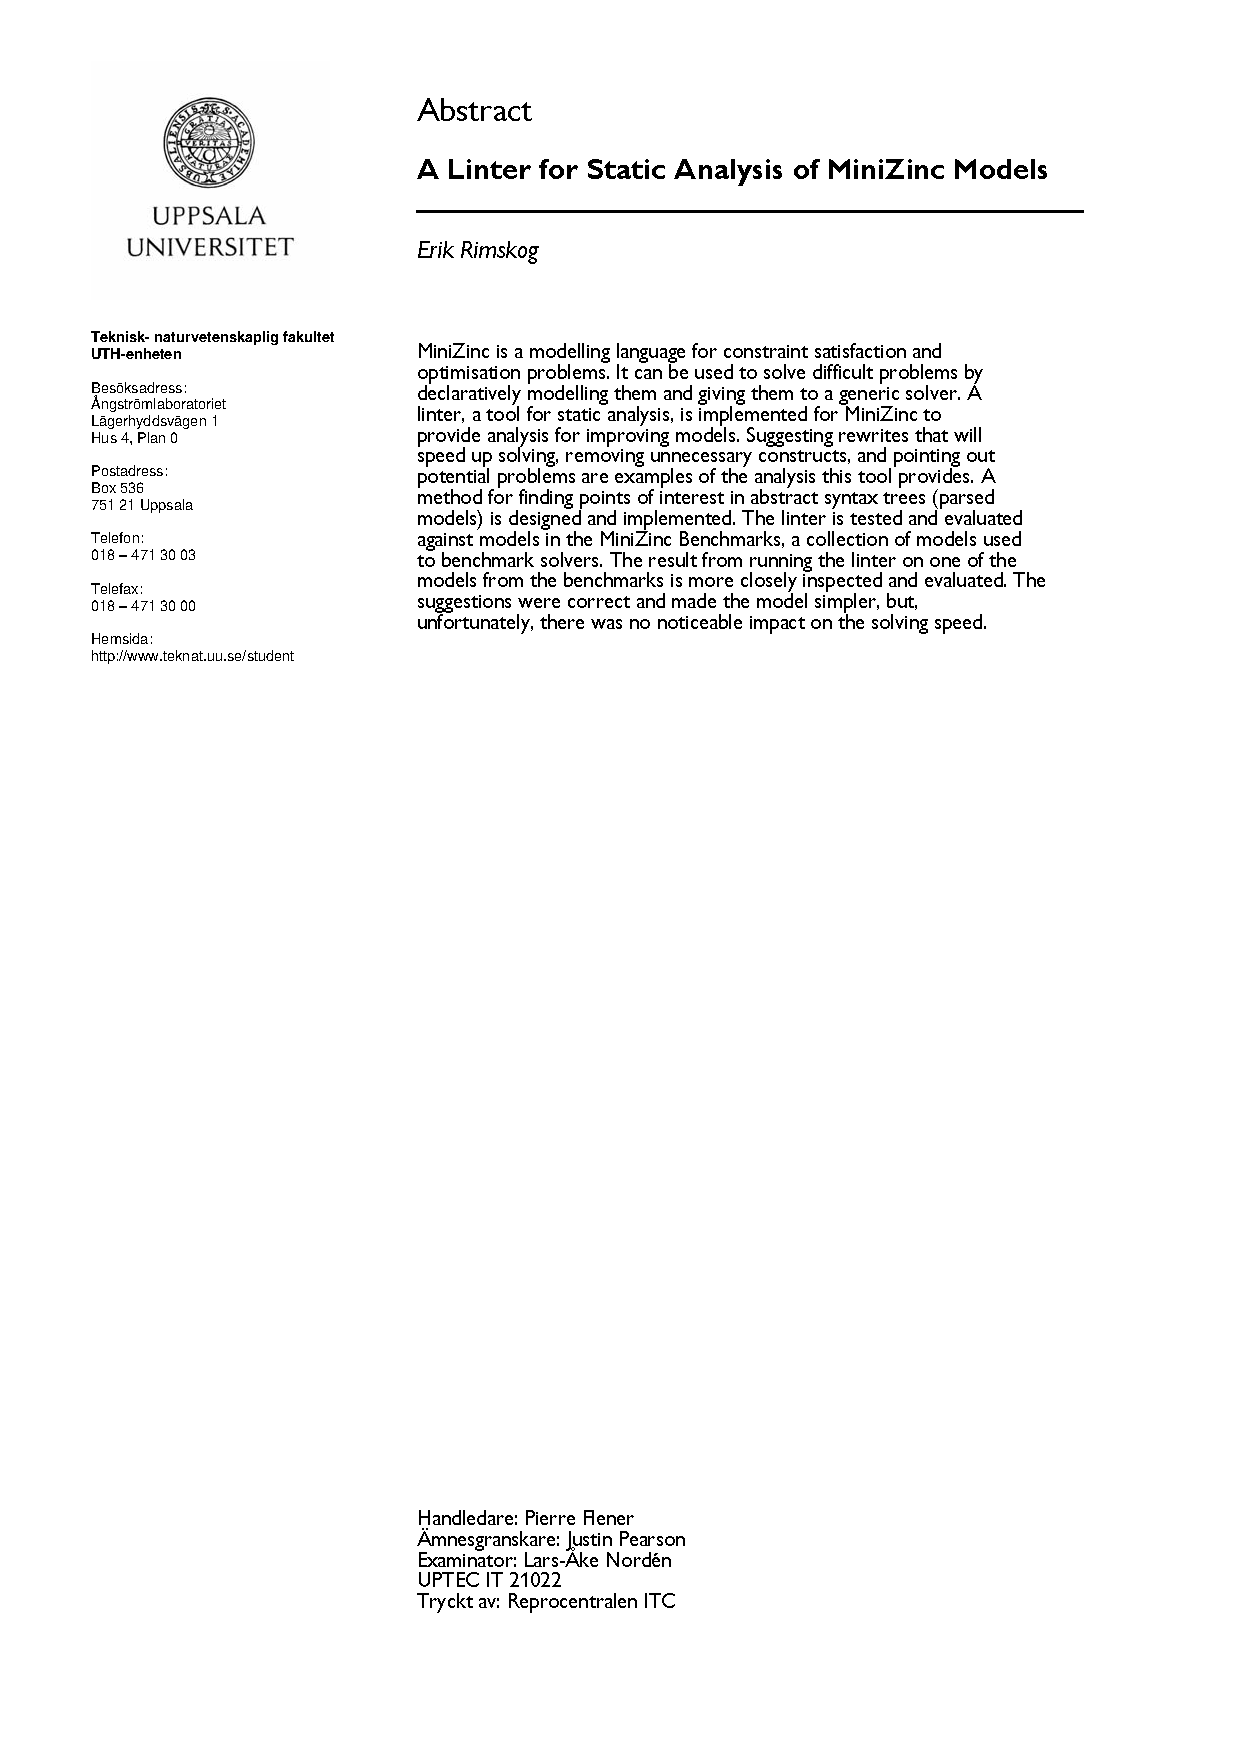
\includepdf[noautoscale=true]{Abstractsida.pdf}
% \begin{abstract}
% MiniZinc is a modelling language for constraint satisfaction and optimisation problems.
% It can be used to solve difficult problems by declaratively modelling them and giving
% them to a generic solver.
% A linter, a tool for static analysis, is implemented for MiniZinc to provide analysis
% for improving models.
% Suggesting rewrites that will speed up solving, removing unnecessary constructs, and
% pointing out potential problems are examples of the analysis this tool provides.
% A method for finding points of interest in abstract syntax trees (parsed models) is designed and implemented.
% The linter is tested and evaluated against models in the MiniZinc Benchmarks,
% a collection of models used to benchmark solvers.
% The result from running the linter on one of the models from the benchmarks is more
% closely inspected and evaluated.
% The suggestions were correct and made the model simpler, but, unfortunately, there was no noticeable impact on the solving speed.
% \end{abstract}

\leblanc

\begin{sammanfattning}
Statisk kodanalys är en metod för att fånga många olika sorters fel och buggar innan
ett program körs. En \emph{linter} är ett samlingsnamn på verktyg som utför
statisk analys, och denna rapport beskriver hur en linter för modelleringsspråket MiniZinc
skapades.

Det finns många kombinatoriska optimeringsproblem som är väldigt svåra att lösa då det inte verkar finnas
några algoritmer
som kan lösa dem på polynomisk tid. Med andra ord finns det inga kända algoritmer som kan lösa
dem problemen ``snabbt'', utan en approximering eller fullständig sökning måste genomföras.
Oftast är en fullständig sökning för långsam, det kan t.o.m.\@ i vissa fall ta flera miljoner år att gå
igenom alla potentiella lösningar, även för relativt små problem.
Två exempel på typiskt svåra problem är schemaläggning och att hitta en ordning att besöka några städer
i som ger den kortaste resvägen.

Det finns generella program som kallas för \emph{lösare} som löser ett problem med hjälp
utav specialiserade algoritmer och metoder som kan hitta en lösning mycket snabbare än att
naivt söka igenom alla lösningar. Lösarna tar oftast en deklarativ beskrivning
av problemet de ska lösa, kallad \emph{modell}. Olika lösare är bra på olika sorters problem, så
flera lösare behöver testas för ett visst problem för att se vilken som är bäst.

MiniZinc är ett verktyg för att modellera kombinatoriska optimeringsproblem på ett universalt vis: en
och samma modell kan användas på flera olika lösare utan att behöva skriva om modellen för
varje (i lösarens egna språk). I MiniZinc kan man modellera problem med hjälp utav beslutsvariabler (\emph{decision
variables}) och begränsningar (\emph{constraints}) på dessa variabler. En lösares uppgift är då att
hitta värden på dessa variabler så att alla begränsingar uppfylls.

Det är lätt att skriva modeller som inte beskriver ett problem i fråga på bästa möjliga
sätt. Konsekvensen blir oftast att det tar längre tid för lösaren att hitta en lösning.
Lintern beskriven i denna rapport letar främst efter vanliga fel som allmänt är kända att
göra det svårare för en lösare att hitta en lösning. Potentiella fel hittas med hjälp utav
en egengjord sökare av abstrakta syntaxträd, vilket är ett formellt sätt att representera källkod på.

Lintern evaluerades i detalj på en utvald modell från \emph{MiniZinc Benchmarks}, en samling av
modeller för prestandamätning. Modellen blev enklare och mer tydlig, med inga märkbara skillnader på lösningstiden.
\end{sammanfattning}

\leblanc

\tableofcontents

\cleardoublepage

% Change to main matter style (arabic page numbers, reset page numbers)
\mainmatter

\section{Introduction}\label{sec:introduktion}
Static analysis on source code is a way to catch many kinds of errors before
a program even is executed.
Bugs, weird special cases, and inefficient code are some of many things that are possible
to statically check, and the tools that do this are called \emph{linters}. 
The history of linters is long. The first linter was lint~\cite{lint}, a tool for
statically checking the code of C~\cite{c1978} programs.

MiniZinc is a declarative solver-independent modelling language for constraint
satisfaction and optimisation problems~\cite{MiniZinc}. The MiniZinc compiler reports
syntax errors and other errors that inhibit a successful compilation. It does not suggest
improvements on the model itself by, e.g., reporting constructs (syntactically valid
sequences of tokens, e.g., \mi{if}-expressions) that should be avoided if possible, or
constructs that are error-prone. This is not surprising, since the MiniZinc compiler's main job is to
process MiniZinc code into FlatZinc code. 
If the construct is valid, then the compiler will
process it, else abort. The goal of this project is to implement a linter that does these
model-improving checks for MiniZinc models. The checks (or rules) implemented are all
described in Section~\ref{sec:rules}.

Constraint satisfaction and optimisation problems have many important applications, such
as scheduling and finding optimal routes. Problems like these can be difficult to solve as
they often do not have a known polynomial-time algorithm. There are programs called
\emph{solvers} that are made to find solutions to problems like this using advanced
algorithms in different technologies, each one good in its own way. Problems are usually
described declaratively as models, where each solver has its own way of specifying them.
MiniZinc is an effort to create a modelling language that can be used with many
solvers, making it a lot easier to try different solvers with the same problem
description. The core of constraint problems consists of constraints and
decision variables. A \emph{decision variable} is a variable with unknown value, and a
solver's task is to find appropriate values for all of these. Each decision variable has a domain, which
is a set of values the variable is allowed to take. The domains can be specified explicitly or,
in some cases, be inferred by the MiniZinc compiler. A \emph{constraint} specifies how
decision variables relate to each other, or what values are allowed, e.g., that one
variable must be greater than another.

Declarative models specify \emph{what} problem to solve, not the exact steps to \emph{how}
it should be solved. It is therefore easy to write inefficient models without knowing it,
since a small edit can greatly affect solving time. A tool to point out potential issues
is attractive to have, especially for beginners, as they might not know what implications
each aspect of a model has and its impact on solving time. For example, the domain of an
integer decision variable should be as small as possible to limit the search space, but if a
domain is not explicitly specified by the modeller, then the domain can potentially be 
as big as the solver can handle, which can slow down solving.

To save time, simplify the implementation, and allow for a possible later integration with
the MiniZinc project, the parser from the MiniZinc project was reused for this project,
specifically its output, namely an abstract syntax tree (AST).
It is generally also good practice to reuse components, there is no need to reinvent the same component again.
An \emph{AST} is a data
structure encoding the formal structure of a program, a MiniZinc model in this case. The
MiniZinc compiler is written in the programming language C++~\cite{cpp}, so this project
is also written in C++ to be able to use the same parser as easily as possible.
Searching
for relevant constructs in the MiniZinc AST is one of the main tasks of this project. More
details on how the AST is searched are described in Section~\ref{sec:impl}.
More detailed explanations on MiniZinc, linters, and parsers are presented in Section~\ref{sec:bakgrund}.

The linter was run on all models in the MiniZinc Benchmarks~\cite{mznbench}, a
big repository of models where most come from earlier MiniZinc
Challenges~\cite{MZN:Challenge}, a competition for solvers. The results are
discussed in Section~\ref{sec:discussion}. An in-depth look into one of the models in
these benchmarks is explored in Section~\ref{sec:nsp}, the suggestions from the linter are
performed and benchmarked.

Possible future work is presented in Section~\ref{sec:future}.

\section{Background}\label{sec:bakgrund}
Section~\ref{sec:mzn} give necessary background information about MiniZinc, what kinds of
problems it can solve, and how a MiniZinc model is written.
What linters are is presented in Section~\ref{sec:bkg:linter}, and in 
Section~\ref{sec:parsing} are parsers and abstract syntax trees explained.

\subsection{MiniZinc}\label{sec:mzn}
A \emph{Combinatorial problem} is a problem of discrete states where some of these states are
solution states~\cite{combopt}. \emph{Combinatorial satisfaction} tries to find these solution states,
while \emph{combinatorial optimisation} tries to find a solution state that minimises or
maximises some quantity associated with each state.

MiniZinc offers a language for modelling combinatorial problems, i.e., constraint satisfaction
and optimisation problems. These are modelled using decision variables and
constraints on those variables~\cite{constraintshandbook}. Each constraint limits the
allowed values of one or more variables.
For example, $x_1 > x_2$, or $x_3 = 3$, etc.
A solution state from all current variable assignments is formed when all constraints are
satisfied.

How a model is processed and used by MiniZinc to produce a solution is explained in Section~\ref{sec:mzn:solvers}.
An introduction to modelling in MiniZinc is presented in Section~\ref{sec:mzn:syntax}.
A full example of a MiniZinc model that solves a ``real'' problem is presented in Section~\ref{sec:tsp}.

\subsubsection{Solvers}\label{sec:mzn:solvers}
There are many solvers and technologies for solving combinatorial optimisation and
satisfaction problems starting from a model thereof, each one good in its own way. Each solver
has its own interface, which makes it time-consuming to compare different
solvers, as the same problem has to be reformulated for each one. MiniZinc~\cite{MiniZinc}
is a tool chain for creating universal models that can be run on any solver MiniZinc
supports, i.e., the \emph{same} model can be used on different solvers without any
rewrites.

A diagram showing how a MiniZinc model is processed to eventually run on a
solver is shown in Figure~\ref{fig:minizinc}. The model itself is written in a text file
that is compiled (or flattened) into something called FlatZinc, a lower-level
representation of the model designed to be easily used by solvers. Each
solver has its own backend, which is a program or library that actually converts the
FlatZinc model into the solver's own model that then can be used by the solver.

\begin{figure}[t]
  \centering
  \begin{tikzpicture}[
  grunka/.style={rectangle,draw,align=center},
  grej/.style={align=center,rectangle},
  solver/.style={minimum width=50pt},
  backend/.style={minimum width=65pt,minimum height=19pt},
  model/.style={minimum width=58pt,minimum height=17pt},
  shorten >=2pt,
  >=stealth'
  ]
  \node [grunka,model] (MZN) at (0, 0) {MiniZinc};
  \node [grunka,model] (DZN) at ($(MZN.center) + (0, -30pt)$) {Instance};
  \node [grunka] (FZN) [right=of MZN] {FlatZinc};
  \node [grunka,backend] (BKN) [right=of FZN] {fzn-gecode};
  \node [grunka,solver] (SLV) [right=of BKN] {Gecode};
  \node [grunka,backend,anchor=west] (BKN2) at ($(BKN.west) + (0,-30pt)$) {fzn-chuffed};
  \node [grunka,solver] (SLV2) at (SLV|-BKN2) {Chuffed};
  \node (ELI) [below=5pt of BKN2] {$\vphantom{\int^0}\smash[t]{\vdots}$};

  \node [above=23pt of MZN,grej,anchor=center] {High-level \\ Model};
  \node [above=23pt of FZN,grej,anchor=center] {Compiled \\ Model};
  \node [above=23pt of BKN,grej,anchor=center] {Backend};
  \node [above=23pt of SLV,grej,anchor=center] {Solver};

  \draw[->] (MZN) edge (FZN)
            (FZN) edge (BKN)
            (BKN) edge (SLV)
            (BKN2) edge (SLV2);
  \draw[->] (DZN.east) -- (FZN.south west);
  \draw[->] ($(FZN.east)!0.7!(BKN.west)$) |- (BKN2);
  \draw[dashed,->] ($(FZN.east)!0.7!(BKN.west)$) |- (BKN2.west|-ELI);

  \verticalline{dotted}{($(MZN.east)!0.5!(FZN.west)$)};
  \verticalline{dotted}{($(FZN.east)!0.5!(BKN.west)$)};
  \verticalline{dotted}{($(BKN.east)!0.5!(SLV.west)$)};
\end{tikzpicture}%

  \caption{How a MiniZinc model gets run by a solver to produce a solution. The high-level
    model is compiled (flattened) into a low-level model that a backend and solver pair
    uses to find solutions.}%
  \label{fig:minizinc}
\end{figure}

MiniZinc models are often divided into two parts: the model itself and an instance. The
model is made generic in the sense that it models some problem, without concrete parameter values. For
example, some model could be modelled in terms of a parameter $n$, but to be solved by a
solver must $n$ have a concrete value. Instances, usually in separate files, provide
concrete values to these parameters. This distinction makes it easy to run the same model
with slightly different values on all parameters. A model is compiled with one instance at a time, so the model has to be
recompiled for each instance.

\subsubsection{Syntax Overview}\label{sec:mzn:syntax}
A MiniZinc model consists primarily of decision variables, constraints,
functions, and \mi{solve}-statements. Decision variables are of various types like
\mi{int}, \mi{bool}, and \mi{float}, and the solver should find appropriate values for them.
Each decision variable has a \emph{domain}, which is a set of values the variable is allowed to take.
Further reduction of allowed values and how the variables should relate to each other are expressed in
constraints. For example, the following listing defines a decision variable \mi{x} of type
\mi{int}, and a constraint that constrains \mi{x} to have a value strictly greater than
five:
\begin{mznnobreak}
var int: x;
constraint x > 5;
\end{mznnobreak}

\begin{sloppypar}
There are two solving modes, specified in a \mi{solve}-statement: satisfaction and optimisation. \emph{Satisfaction}
finds values for all decision variables such that all constraints are satisfied, and
\emph{optimisation} additionally minimises or maximises some decision variable or expression.
For example, adding \mi{solve minimize x} to the listing above would create a
model that tries to find the smallest integer value greater than five, which is
six. Adding \mi{solve satisfy} would instead find \emph{some} integer greater than
five. An optional \emph{search annotation} can be specified on a \mi{solve}-statement, specifying
a hint that some solvers take into account. The following is an annotation that
hints how \mi{x} should be searched for:
\end{sloppypar}
\begin{mznnobreak}
:: int_search([x], input_order, indomain_min)
\end{mznnobreak}
The first argument is the array of variables to specify a hint for, the
second argument gives the order in which the variables in the array should be searched for,
and the last argument specifies how the chosen variables should be constrained given their
current computed domains. In this example, \mi{indomain_min}, specifies that the minimum
value in the current domain should be tried first.

Variables that are fixed to a given value are in MiniZinc called \emph{parameters}.
A parameter is declared with \mi{par}, or no keyword at all, instead of \mi{var}.
These parameters are useful since they can be used to generalise a model, and to give descriptive names to constants.
For example, the above listing can be rewritten with a parameter as follows:
\begin{mznnobreak}
int: n = 5;
var int: x;
constraint x > n;
\end{mznnobreak}
Now the value of \mi{n} can easily be changed to solve a different instance.

This model can be separated into an instance file and a model file by giving
the model the declaration \mi{int: n} and the
instance file the assignment \mi{n = 5}. Multiple instance files can be created
for a single model, which makes it possible to change all parameters at once.

\emph{Arrays} allow for a variable amount of variables. The listing below shows an array \mi{xs}
consisting of five integer variables. A variable in the array can be accessed separately with
a special syntax. For example, the first variable can be accessed with
\mi{xs[1]}.
To access all variables in an array at once, the built-in function \mi{forall} can be used.
The listing below uses this to constrain all variables in the array to be strictly greater
than five, it is like writing a universal quantification: $\forall x \in xs : x > 5$.
\begin{mznnobreak}
array[1..5] of var int: xs;
constraint forall(i in 1..5)(xs[i] > 5);
\end{mznnobreak}

The \mi{forall} constraint above is syntactic sugar (alternate syntax) for the \mi{forall}-function on a list comprehension.
A \emph{list comprehension} is a way to specify a list in a similar manner to set-builder notation:
one or more sets or arrays are enumerated, and the elements satisfying an optional Boolean expression are included in the resulting list;
the values included are given by an expression on the enumerated elements.
An example comprehension that creates a list of squares of even numbers is:
\begin{mznnobreak}
[x*x | x in 1..50 where x mod 2 = 0]
\end{mznnobreak}

The \mi{forall} above can thus also be written as:
\begin{mznnobreak}
constraint forall([xs[i] > 5 | i in 1..5]);
\end{mznnobreak}

The final feature that will be covered here is functions. Functions allow the modeller to
reuse the same code in multiple places. A \emph{function} has a return value, a function body, and zero or more
arguments, all of which can have the same possible types as
decision variables (\mi{int} etc.). The following listing is a declaration and usage of a function that takes a decision variable as
an argument and returns a decision variable:
\begin{mznnobreak}
function var int: a_name(var int: x) = <@\textit{<some expression>}@>;
constraint a_name(x) < 69;
\end{mznnobreak}

\begin{sloppypar}
Some functions called global constraints are special. A \emph{global constraint} is a
function defined in a standard library for high-level modelling abstractions. There is
a global constraint called \mi{all_different} that constrains all variables in an array to
all take different values from each other. Many solvers implement special inference algorithms for
global constraints, which means that they can reason a lot better about them.
Using a global constraint is preferred over directly using its definition.
For example, it is preferred to use \mi{all_different(xs)} instead of
\mi{forall(i,j in index_set(xs) where i < j) (xs[i]!=xs[j])}.
\end{sloppypar}

\subsubsection{Travelling Salesperson Problem}\label{sec:tsp}

An example of combinatorial optimisation is the travelling salesperson problem (TSP) where a
seller wants to travel to $n \in \elnaturale^+$ towns in a cyclic order that minimises the total
distance travelled. Here, the solution states are all orderings that visit every town once and 
return to the start town, the quantity to minimise is the total distance.

The following is an example of how TSP can be modelled in MiniZinc,
its instance is illustrated in Figure~\ref{fig:tsp}:
\begin{mznbreak}
include "globals.mzn";
int: n = 4;
set of int: ns = 1..n;
array[ns,ns] of int: dist =
  [| 0,15,20,26
   |15, 0, 5,12
   |20, 5, 0, 5
   |26,12, 5, 0|];
array[ns] of var ns: next;
constraint circuit(next);
solve minimize sum(i in ns)(dist[i,next[i]]);
\end{mznbreak}

\begin{figure}[t]
  \centering
  \begin{figure}[ht]
  \centering
  \begin{tikzpicture}[
    city/.style={draw, circle, minimum size=9mm},
    arr/.style={rectangle, minimum size=0.4cm},
    Arr/.style={-{Stealth}},
    ]
    \node (SLA) at (-3, -1) [city, label=above:Sala] {1};
    \node (HBY) at (2, 0) [city, label=above:Heby] {2};
    \node (MGA) at (5, -0.2) [city, label=above:Morgongåva] {3};
    \node (VIT) at (7.3, -1.4) [city, label=above:Vittinge] {4};

    \draw (SLA) edge[Arr,above, near start] node {20} (MGA)
          (MGA) edge[Arr,above] node {5} (HBY)
          (HBY) edge[Arr,above, near end] node {12} (VIT)
          (VIT) edge[Arr,below] node {26} (SLA);

    \node (A1) at (0, -3) [arr, label=north:1] {3};
    \node (A2) [arr, right=0 of A1, label=north:2] {4};
    \node (A3) [arr, right=0 of A2, label=north:3] {2};
    \node (A4) [arr, right=0 of A3, label=north:4] {1};
    \draw (A1.north west) -- (A4.north east) -- (A4.south east) -- (A1.south west) -- cycle;
    \draw (A1.north east) -- (A1.south east)
          (A2.north east) -- (A2.south east)
          (A3.north east) -- (A3.south east);

    \node [right=of A4] {$\sum = \SI{63}{km}$};
  \end{tikzpicture}
  \caption{Example instance of Travelling Salesman Problem with $n=4$ cities. The state is
    $\langle 3,4,2,1 \rangle$, which means that after city 1 is city 3 visited, after
    city 2 is city 4 visitied etc. The total distance travelled is \SI{63}{km}. Only the
    paths for the current route are shown.}%
  \label{fig:tsp}
\end{figure}

  \caption{Example instance and non-optimal solution of TSP with $n=4$ towns. The state is
    $\langle 3,4,2,1 \rangle$, which means that town 3 is visited after town 1, town 4 is
    visited after town 2, etc. The total distance travelled is \SI{63}{km}. Only the paths
    for the solution route are shown.}%
  \label{fig:tsp}
\end{figure}

TSP could be modelled with a list of \mi{n} integers, from 1 to \mi{n}, where each
integer represents a town (line~2 and line~3). A 2D-array, or matrix, is constructed on
line~4 with the distances between all pairs of towns. 
The distance between towns \mi{i} and \mi{j} is given by \mi{dist[i,j]}.
The actual route to travel is encoded as an array on line~9, that is the decision variables.
The value of \mi{next[i]} is what town to visit next; e.g., \mi{next[1] = 2} means that
town~2 shall be travelled to after town~1. The global constraint \mi{circuit} on line~10
is constraining \mi{next} to complete a circuit (cyclic path) between all towns. An example of a
circuit is $\langle 2,3,4,1 \rangle$, and an invalid circuit is $\langle 1,1,2,3 \rangle$.
The global constraint must be imported from the standard library: see line~1. Finally,
line~11 specifies the expression to minimise, which is the total distance in this case. The
distance from a town to itself can be anything as \mi{circuit} prohibits a town to have
itself as next destination.

\subsection{Linters}\label{sec:bkg:linter}
% Lint is a program for doing static code analysis of C programs~\cite{lint}. The term
% \emph{linter} originates from this program and is nowadays a general term for any tool
% that performs static code analysis, except for things a compiler typically does, like
% syntax analysis and semantic analysis (type checking). Static in this context means that
% the analysis is done on the source code itself, without executing it.

A \emph{linter} is a program for doing static analysis of source code, \emph{static} meaning that
the analysis is done without running the program. The term linter originates from a
program called lint~\cite{lint}, a tool for analysing C~\cite{c1978} programs. A linter can look for
bugs, enforce a certain code style, find a type of improvement, find error-prone
constructs, point out special cases, etc. Compilers also do static analysis when they are
compiling, e.g., syntax analysis (whether a sequence of characters encodes a valid
construct) and semantic analysis (type checking, etc.).

A compiler's main job is to convert source code into some other source code, usually machine
code, and it is probably aiming at doing so as fast as possible. A compiler generally only
does the minimum amount of analysis required to determine if the given source code is
legal, i.e., following the language's standard. Even if a program is legal does not mean
it is good: it could crash immediately on start up. Linters take a more leisurely view and
try to see whether there are any potential problems with the otherwise legal program. A
linter could look for uninitialised pointers in C programs that are dereferenced (as that would
most likely make the program crash) and warn about them. Finding uses of variables that
have not been set to a value is something the original lint does~\cite{lint}. Another
distinction is that linters are not as precise as compilers. Linters provide
\emph{suggestions}: it is fine if they are wrong, and the worst thing that can happen is that
the user gets annoyed by false positives. A compiler, in contrast, should never be wrong: it
should always be certain about its conclusions, as it might not produce correct programs
otherwise.

There also are linters and other static analysis tools for
interpreted programming languages, i.e., languages whose programs are run ``as is'' without compiling them first. Python
is an example of a dynamically typed (which means that types are determined at runtime) and interpreted
language. It is possible to put optional type information into a Python program and have a
third-party program like mypy~\cite{mypy} do static type checking; mypy is not
a linter as it performs type checking, something a compiler typically does.

The checks a linter does are typically called \emph{rules}, and different linters have
different ways of specifying them. The JavaScript linter ESLint~\cite{ESLint} allows the users
to create their own rules in separate JavaScript files, alongside the built-in ones.
Since JavaScript is interpreted, new user-specified rules can be added relatively easily:
they are loaded as any other file.
A rule in ESLint
consists of a pattern match on the AST and a function
that will do additional checks to see whether it is an actual match or not.
The rules in this project are structured in the same
manner, except that the part that pattern matches is not as powerful. The one in ESLint can
find arbitrary sub-trees, while the one in this project can only find paths (sub-trees that
are a line) in the AST.

Clippy~\cite{Clippy} is a linter for the programming language Rust~\cite{rustlang}. Rust
is a compiled language and rules to Clippy are specified as Rust source code. 
This means that the whole Clippy project has to be recompiled whenever a new rule is added,
similar to this project.
Clippy's rules are specified similarly to ESLint, with the difference
on how the AST is traversed. Each Clippy rule has special functions that are called on
various items in the language, like function and \cpp{struct} declarations. Each of these
special functions determines if there is anything relevant to report to the user for that
item.

The linter hlint~\cite{hlint} is for the compiled functional language
Haskell~\cite{haskell}. It specifies rules in YAML, a typical format for
general configuration, not in Haskell or a custom-made language. This is possible since the rules
for hlint are relatively simple: they are pattern matches against the Haskell source code.
The suggested rewrite is also specified as plain Haskell code. One example rule finds
\texttt{not (a == b)} and suggests rewriting it to \texttt{a /= b}, as the rewrite is shorter
and handles \texttt{NaN} (short for ``not a number'', typically used for representing invalid results) correctly.

Rules in linters are usually divided into several categories so they can be collectively disabled or
enabled more easily. An example of this could be to disable all rules about white space
and indentation. They also usually have unique identification numbers or names so that they can
be individually disabled if desired. The rules in this project have unique IDs and each rule belongs
to some category.
The available categories in this project are:
\begin{description}[noitemsep]
  \item[Challenge] rules that enforce the rules of the MiniZinc Challenge
  \item[Style] rules that suggest stylistic changes
  \item[Unsure] rules that eagerly mark things that in general are bad
  \item[Performance] rules that suggest changes that can increase performance
  \item[Redundant] rules that suggest removing redundant or unused things
\end{description}

The tool ShellCheck~\cite{shellcheck} is a linter for shell scripts like
bash~\cite{bash}. One rule it has checks for incorrect usage of \texttt{\$@}.
The construct \texttt{"\$@"} expands to all arguments passed to the
current script, which is useful if all arguments should be processed to determine the script's
behaviour. The quotes are vital, since the expression without them will perform additional
word splitting on the arguments, which is not desired in the majority of cases. Consider a script called with the
arguments ``-f'' and ``my cool model.mzn''. The expression \texttt{"\$@"} will expand
into the same arguments, i.e., ``-f'' and ``my cool model.mzn''. However, without quotes, i.e.,
\texttt{\$@}, it will instead expand to ``-f'', ``my'', ``cool'', and ``model.mzn'', because each argument
has been split into words. The lint
rule called ``SC2068'' in ShellCheck does exactly this analysis.

\subsection{Parsing and Abstract Syntax Trees}\label{sec:parsing}
To be able to process source code, or models, in text format, it is common to parse them
into some kind of data structure. There are many tools available called \emph{parser
generators}, which are programs that take some kind of formal description of the
language to be parsed and generate source code in some programming language for a parser.
MiniZinc uses a parser generator called Bison~\cite{flexbison}, which is a generator that
can generate C++ code, the same language that MiniZinc is written in.

The output of a parser is often an abstract syntax tree (AST), an example of which is
given in Figure~\ref{fig:bkg:ast}. An AST is representing the formal structure of the
source code as nodes with sub-nodes, i.e., a tree. A function in C++ could
,for example, be represented as a node with a child for every statement in that function.
Each statement is itself a tree, encoding whatever that statement represents. The
information about the arguments and the return type could be stored in the node itself or
as yet more children: there are many ways to design an AST.

\begin{figure}[t]
  \centering
  \begin{tikzpicture}[AST, eval/.style={red, font=\footnotesize}]
  \node (l) at (0, 0) {*}
    child {node {0}}
    child {node {+}
      child {node {2}}
      child {node {$f$}
        child {node {3}}}};

  \node [eval, above right=-6pt and 0pt of l-2-2-1] {3};
  \node [eval, above right=-6pt and 0pt of l-2-2] {3};
  \node [eval, above right=-6pt and 0pt of l-2-1] {2};
  \node [eval, above right=-6pt and 0pt of l-2] {5};
  \node [eval, above right=-6pt and 0pt of l-1] {0};
  \node [eval, above right=-6pt and 0pt of l] {0};

  \node (r) at (6, 0) {+}
    child {node {*}
      child {node {0}}
      child {node {2}}}
    child {node {$f$}
      child {node {3}}};

  \node [eval, above right=-6pt and 0pt of r-2-1] {3};
  \node [eval, above right=-6pt and 0pt of r-2] {3};
  \node [eval, above right=-6pt and 0pt of r-1-1] {0};
  \node [eval, above right=-6pt and 0pt of r-1-2] {2};
  \node [eval, above right=-6pt and 0pt of r-1] {0};
  \node [eval, above right=-6pt and 0pt of r] {3};
\end{tikzpicture}

  \caption{On the left is a possible tree of the expression $0\cdot(2+f(3))$. The right one
    is a possible tree of the expression $(0 \cdot 2)+f(3)$. The asterisk in the trees
    represents multiplication. The different placements of the parentheses change what the
    generated tree looks like. The red numbers on the sides represent what each sub-tree
    evaluates to if $f(x) = x$.}%
  \label{fig:bkg:ast}
\end{figure}

An AST is abstract in the sense that it does not encode everything in the original code.
Things like parentheses in mathematical expressions are often implicitly encoded by the
position each operator has in the tree.
Two example ASTs of mathematical expressions are shown in Figure~\ref{fig:bkg:ast}.
Those trees are evaluated bottom up, and each node's value is
its operation applied to the results of its child nodes. Nodes high up in the tree are
therefore evaluated \emph{after} their child nodes, which means that sub-expressions that
should be evaluated first, like expressions in parentheses, are placed further down in the
tree.

\section{Implementation}\label{sec:impl}
This project is implemented using C++~\cite{cpp}, a compiled programming language with
performance as a main design goal. The parser that the MiniZinc project is
using was reused in this project, both to save time and to simplify the implementation.
% This project will only analyse the Abstract Syntax
% Tree (AST) given from the parser, so it is unnecessary to write a new parser which would
% do the same thing.
Only the abstract syntax tree (AST) will be searched: no extensions or
modifications are thus needed, allowing the parser to be reused as is.
Using the same AST would also make it possible to reuse other utilities
present in the MiniZinc compiler, such as the type checker and pretty printer (converting
the AST back to nicely formatted code). Multiple complicated aspects of the language were
provided for free as a consequence of reusing the parser, and were thus not needed to be
re-implemented. One such aspect is \emph{function
resolution}, i.e., the rules and logic behind what function definition to use given a name
and some arguments. Another reason
for reusing the parser is to make a potential integration into the original project easier,
as one parser is easier to maintain than two.

The MiniZinc
compiler is written in C++, so creating this project in the
same language was a natural choice. C++ comes in several standards, and C++17 is the one
chosen for this project as that was the latest one that all major compilers fully supported at
the time this project started. The MiniZinc version is 2.5.5 as, again, that was the
latest version when this project started.

An overview of how the linter itself is structured is explained in
Section~\ref{sec:impl:structure}. The AST searcher will be explained in detail in
Section~\ref{sec:searcher}. How rules are added is explained in Section~\ref{sec:impl:rules}.

\subsection{Application Structure}\label{sec:impl:structure}
\begin{figure}[t]
  \centering
  \smallskip%
  \begin{figure}[ht]
\centering
\smallskip%
\begin{tikzpicture}[
  blackrekt/.style={draw, rectangle},
  number/.style={auto,draw,circle,solid,inner sep=1pt,outer sep=3pt, node font=\scriptsize, very thin},
]
  \node (LE) at (0, 0) {\cpp{LintEnv}};
  \node (IP) [blackrekt, below=0.2 of LE.south west, anchor=north west] {Include paths};
  \node (AST) [blackrekt, right=0.2 of IP] {AST};
  \node (RES) [double copy shadow={shadow xshift=4pt, shadow yshift=0}, fill=white, blackrekt, below=0.2 of IP.south west, anchor=north west] {\cpp{LintResult}};
  \node (BOX) [fit=(LE) (IP) (AST) (RES), blackrekt] {};

  \newcommand{\lintrule}[2]{
    \node (#1) at #2 {\cpp{LintRule}};
    \draw[fill=white] (#1.north west) +(0, 0.5) -| ($(#1.north west)!0.3!(#1.north east)$)
    -- ($(#1.north west)!0.7!(#1.north east)$) |- ($(#1.north east) + (0, 0.5)$)
    -- (#1.south east) -- (#1.south west) -- cycle;
  }
  \foreach \y in {-4.2, -4.1, -4} \lintrule{LR1}{(-\y, \y)};
  \node (PR1) at (4, -4) {\cpp{LintRule}};
  \draw[big arrow, shorten >=8pt] (BOX) edge[out=0, in=90] node [number, near start] {1} (LR1);
  \draw[big arrow, dashed] (LR1) edge[out=180,
  in=-90] node [number] {2} ($(BOX.south) + (0.5, 0)$);

  \node (PRT) [rectangle, align=left, draw=black, line width=1mm, rounded corners, inner sep=2mm] at (-3, -3.6) {\texttt{\textbf{\Large >\_}} \\ Stdout printer};
  \draw [big arrow] (RES) edge[in=90,out=180,looseness=1.3] node [number] {3} (PRT);

\end{tikzpicture}%
\smallskip%
\caption{Illustration for the main execution of the linter. The \cpp{LintEnv} is given as
  an argument to each \cpp{LintRule} (1). Each rule will analyse the AST and write its
  results back to a list inside \cpp{LintEnv} (2). When all rules have been processed, is
  the list of all results given to a function that will output them back to the user
  (3).}%
\label{fig:overview}
\end{figure}

  \smallskip%
  \caption{Illustration for the main execution of the linter. The \cpp{LintEnv} is given as
    an argument to each \cpp{LintRule} (1). Each rule will analyse the AST and write its
    results back to a list inside \cpp{LintEnv} (2). When all rules have been processed, 
    the list of all results is given to a function that will output them to the user
    (3).}%
  \label{fig:overview}
\end{figure}

The overall structure of the linter is illustrated in Figure~\ref{fig:overview} and
everything following here will be illustrated in that figure. The most important component
of this linter is a base class called \cpp{LintRule}. Each rule
is its own class that inherits from \cpp{LintRule}. Each rule
consists of: a unique ID, what category it belongs to,
a name, and a method that accepts a model that returns the result of the rule, if any.
This model argument is an object of the class \cpp{Model}, i.e., the AST from the parser
in the MiniZinc project.
The ID and category are used for filtering which rules to use, and the name is used
for printing purposes. Each rule performs its analysis by first searching in the AST for a
relevant construct, which, for example, could be a variable used inside the condition of an
\mi{if}-expression, followed by multiple checks or other processing to figure out whether
this construct should be reported to the user or not. They do this search by using a
custom searcher described in Section~\ref{sec:searcher} below.

\begin{sloppypar}
The rules do not take the AST directly: they take it wrapped in a class called
\cpp{LintEnv}. This class contains a lot of helper functions that each rule interacts with
directly. The class \cpp{LintEnv} contains, aside from the AST, a list called \emph{include paths}.
This list contains file paths to directories that contain library files.
MiniZinc comes with a standard library that MiniZinc functions are defined in (e.g., global constraints), and include paths help the linter to find them.
The class \cpp{LintEnv} also contain all results and methods to create new results. The final thing
this class does is caching the results from searches that are common, i.e., multiple rules performs them.
One such search is finding all user-defined variables, both top-level ones and those defined in \mi{let}-expressions.
\end{sloppypar}

Each result is recorded in a class called \cpp{LintResult}. That class hold the relevant data
for a result, which is: what rule it came from, the file position (line and column) for where it
matched, an explanatory message, and an optional recommended rewrite. These results are
then given to a function that will present them to the user. It can be
printed to standard output in a human-readable form, or converted to the JSON-format and
given to an IDE, or something else.

These are all the relevant components for a high-level overview of the linter. A
typical execution of the linter in terms of these components is as follows:
\begin{enumerate}
  \item Gather options and model files from the arguments of the process.
  \item Parse to file into a \cpp{Model} class (AST); abort if errors occurred.
  \item Type check the AST; abort if errors occurred.
  \item Construct a \cpp{LintEnv} object.
  \item Iterate through all \cpp{LintRule} and perform their analysis, saving their
  results to \cpp{LintEnv}.
  \item Give the list of all \cpp{LintResult} to a function that will output them to, e.g.,
  the terminal.
\end{enumerate}

\subsection{Abstract Syntax Tree Searcher}\label{sec:searcher}
This project uses a custom-made algorithm for finding relevant positions of interest in a
MiniZinc abstract syntax tree (AST). Many rules require more complex searches than the
matching of single nodes in the AST, e.g., ``find \mi{x=3} anywhere inside constraints
except for in the \mi{else}-clause of \mi{if}-expressions'' instead of ``find all \mi{if}-expressions''.
This algorithm is called \emph{searcher}, and it simplifies the process of searching with complex search queries in the AST.
An alternative
approach would be to use what the MiniZinc project already uses for processing the
AST, namely visitors. A \emph{visitor} would process the tree by running various functions on each
node, chosen by the type of the node~\cite[p.~331]{DesignPatterns94}. It would be easy to find
single nodes of interest using visitors, but it would be verbose to find
more complicated constructs. 

How the ASTs in MiniZinc looks like is explained in Section~\ref{sec:searcher:ast}.
How the query language for the searcher works is explained in Section~\ref{sec:paths}.
The algorithm behind the searcher is explained in Section~\ref{sec:algo}, and its run-time complexity is
derived in Section~\ref{sec:algo:anal}.
How more precise searches can be performed is explained in Section~\ref{sec:filter:stdlib}.
Finally, how the C++ implementation looks like is presented in Section~\ref{sec:searcher:cpp}.

\subsubsection{MiniZinc Abstract Syntax Tree}\label{sec:searcher:ast}
\begin{figure}[t]
  \centering
  \newif\ifshowastnumbers\showastnumberstrue
  \newcounter{asdasd}

\begin{figure}[ht]
\centering
\begin{tikzpicture}[
label distance=-10pt,
every label/.style={blue},
lbl/.style={label=160:{\stepcounter{asdasd}\arabic{asdasd}}}
]
  \node at (0, 0) {\mi{constraint}} [sibling distance=60pt]
  child {node[lbl] {\cpp{BinOp} =}
    child {node[lbl] {\cpp{BinOp} +}
      child {node[lbl] (X) {\cpp{Id} ``x''}}
      child {node[lbl] {\cpp{IntLit} 42}}
    }
    child {node[lbl] {\cpp{Id} ``y''}}
  };

  \node (VX) at (6.5, 0) {\mi{var int: x}} [level 2/.style={sibling distance=140pt}, level 3/.style={sibling distance=65pt}]
  child {node[lbl] {\cpp{BinOp} +}
    child {node[lbl] {\cpp{BinOp} +}
      child {node[lbl] {\cpp{IntLit} 1}}
      child {node[lbl] {\cpp{IntLit} 1}}
    }
    child {node[label=177:{\stepcounter{asdasd}\arabic{asdasd}}] {\cpp{BinOp} +}
      child {node[lbl] {\cpp{IntLit} 1}}
      child {node[lbl] {\cpp{IntLit} 1}}
    }
  };

  \draw[-{Straight Barb[scale=1.3]},dashed] plot [smooth] coordinates {(X.south) ($(X.south) + (3, -0.3)$) ($(VX.west) + (-1.2, -0.5)$) (VX.west)};
\end{tikzpicture}
\caption{Illustration of two ASTs. The left one corresponds to \mi{constraint x+42=y},
  and the right one corresponds to \mi{var int: x=1+1+1+1}. The blue numbers are
  for referring to the nodes more easily and are not a part of the AST. The \mi{Id} at
  node 3 has a pointer to its declaration. \cpp{BinOp} is short for ``binary operation'',
  \cpp{Id} is short for ``identifier'' and lastly \cpp{IntLit} is short for ``integer
  literal''. These three are names of classes from MiniZinc.}%
\label{fig:ast:searcher}
\end{figure}

  \caption{Illustration of two ASTs. The left one corresponds to \mi{constraint x+42=y},
    and the right one corresponds to \mi{var int: x=1+1+1+1}. The blue numbers are
    for referring to the nodes more easily and are not a part of the AST. The \mi{Id} at
    node 3 has a pointer (the dashed arrow) to its declaration. \cpp{BinOp} is short for ``binary operation'',
    \cpp{Id} is short for ``identifier'', and lastly \cpp{IntLit} is short for ``integer
    literal''. These three are names of classes from MiniZinc.}%
  \label{fig:ast:searcher}
\end{figure}

The output of the MiniZinc parser is an object of the class \cpp{Model}. It is not strictly
an abstract syntax \emph{tree}, but more like an abstract syntax
\emph{graph}. That is because the \cpp{model}-class contains several ASTs that can refer to each other.
An illustration of this graph is shown in Figure~\ref{fig:ast:searcher}.
The \cpp{Model}-class contains a list of all top-level items in a model, such as: constraints, variable
declarations, and functions. Each of those contains one or more expressions. An \emph{expression} is
something that can be evaluated to some value if every variable it contains has a known value. 
For example, the expression \mi{1+1} evaluates to the integer \mi{2}.
There are several \emph{types} that AST nodes in an expression can be of, namely one for each concept,
examples being addition, implication, comprehension, and identifier.
Each expression is not strictly a tree either since, for example,
an \cpp{Id}-node, which represents an identifier like ``x'', has a pointer to the variable
declaration it is referring to. The searcher explained here will actually search in these
top-level ASTs individually, but the whole model will be referred to as one AST for
simplicity.

Each expression saves where it came from, namely the filename, beginning line, end
line, beginning column, and end column. If an expression does not come directly from a file,
but was auto generated by the compiler, then it is marked as ``introduced'' instead.

\subsubsection{Query Language}\label{sec:paths}
The searcher finds paths in the AST from a specification, called a \emph{query}.
A query consists of two parts: the first one being what top-level items to search in, and the
second one being what target path (explained below) to search for in each searched top-level item.
Each type of top-level item can either be searched or not, decided by a Boolean value associated with each type.

In a tree, a \emph{path} is a sequence of
nodes $n_1, n_2, \dots ,n_m$, where $m \in \elnaturale^+$ and $n_i$ is a direct child of $n_{i-1}$ for
all $i \in \{2,\dots,m\}$.
A \emph{target path}, given as a non-empty sequence of what are called targets, 
specifies what a path to search for looks like.
A \emph{target} is denoted by $T_{R,N}$, where $N$ is what type of AST node to match
against and~$R \in \{U,D\}$ specifies how a node matched by a target relates to the node
matched by the previous target in the sequence: the value $D$ (for `direct') means that the
node matched should be a direct child of the previous match, and $U$ (for `under') means
that the node can be a child at any depth of the previous match. If $T_{R,N}$ is the first target
in the sequence, then $R$ is not referring to the previous match, but to an implicit dummy node
that only has the root as child:
the value $D$ in this case means that the match has to be the root of the tree, and $U$ means
that the match can occur anywhere. 
The root refers to the root node of an expression, not to a top-level item since it is
not included in the search for paths.

For example, the target path $\langle T_{D,=} \; T_{U,+} \rangle$ will match a \cpp{BinOp}~=
at the root of the AST, and then match a \cpp{BinOp}~+ anywhere on either the left-hand
side or right-hand side of the equal-node. Taking the left tree in
Figure~\ref{fig:ast:searcher} as an example, this target path will give only the path
$\langle 1,2 \rangle$ as a match.

Another example is the target path
$\langle T_{U,+} \; T_{U,\text{\mi{IntLit}}} \rangle$: it will match a plus-node
anywhere that has an integer literal somewhere under it. The left tree in
Figure~\ref{fig:ast:searcher} has one path matching this, namely $\langle 2, 4 \rangle$.
The right tree on the same figure has several matches, namely
$\langle 6, 7, 8 \rangle$, $\langle 6, 7, 9 \rangle$, $\langle 6, 10, 11 \rangle$,
$\langle 6, 10, 12 \rangle$, $\langle 7, 8 \rangle$, $\langle 7, 9 \rangle$,
$\langle 10, 11 \rangle$, and $\langle 10, 12 \rangle$.

\subsubsection{Algorithm}\label{sec:algo}
The algorithm to perform the path matching described in Section~\ref{sec:paths} is a backtracking
algorithm. It will do a depth-first search (DFS) to iterate over all paths in the AST. If
the algorithm at some point deduces that the current path cannot possibly produce a full
match for a target path, then it will stop searching that path and backtrack to an
earlier point and try a different path.

The pseudo-code is displayed in Algorithm~\ref{alg:searcher} on page~\pageref{alg:searcher}. The algorithm is given an
AST of an expression with $m \in \elnaturale^+$ nodes and a target path $t_1, t_2, \dots, t_n$, where $n \in \elnaturale^+$.
The algorithm maintains a stack $D$ for a DFS on the
AST, and another stack $P$ that contains the current path the DFS is on. Nodes get pushed
to $P$ as they are discovered, but the algorithm must also know when to pop them from $P$. For this,
the algorithm
has to know when a particular node's children have been searched. Let us say that the DFS
popped a new node $x$ from $D$: it will then push $x$ to $P$ to update the current path, but it will
also push it back to $D$, as a marker, followed by all direct children of $x$. Now, if at any point later in
the search $x$ gets popped again from $D$ and the top element of $P$ also is $x$, then the DFS
algorithm knows that all sub-nodes of $x$ have been processed and that it is now okay to pop $P$.

Some nodes in $P$ will be matched nodes by some target path $t_i$, and some will be ``nodes on the way''
when $U$ is used. Only the matched nodes are of interest, so yet another stack $H$
will keep track of the same path as $P$ but only store nodes matched directly from all $t_i$.
The stack $H$ is therefore a sub-stack of $P$, and
$H$ will have a maximum size of $n$, while $P$ will have a maximum size equal to
the height of the AST.

A variable $1 \leq x \leq n+1$ is used to keep track of the progress in the target path: the value of $x$ is the index of
the next \emph{unmatched} target to find. If $x = n+1$, then all targets are matched.
The result in $H$, when this condition is met, can be saved in a list to later be returned, or it can be processed immediately
before the next match is searched for. The latter case was used in this project.

\begin{algorithm}[p]
\begin{algorithmic}[1]
\Procedure{Searcher}{$\mathit{AST}, t_1,\dots,t_n$}
  \State {$D\gets \mathtt{root}(\mathit{AST}) \quad P\gets \emptyset \quad H\gets \emptyset$}
  \Comment {Initialise all the stacks}
  \State {$x\gets 1$}\Comment{$t_1$ is the next target to match}
  \While {$D \neq \emptyset$}
    \State $d\gets \mathtt{pop}(D)$\Comment{the currently visited node}
    \If {$d = \mathtt{top}(P)$}\Comment{A marker was popped}
      \State $\mathtt{pop}(P)$\Comment{$d$ is no longer on the current path}
      \If {$d = \mathtt{top}(H)$}
        \State $\mathtt{pop}(H)$
        \State $x\gets x-1$
        \If {$t_x$ is $U$}\Comment{This step forces $d$ to be unmatched, this allows}
          \Statex\Comment{other nodes under $d$ to be matched against $t_x$}
          \State Push $d$ to $P$ and $D$, and also push all direct children of $d$ to $D$
        \EndIf
      \EndIf
      \Continue
    \EndIf
    \If {$t_x$ matches $d$}
      \State $x\gets x+1$
      \State Push $d$ to $H$
    \Else
      \If {$t_x$ is $U$}\Comment{$t_x$ had to match directly after $t_{x-1}$, but it did not}
        \Continue
      \EndIf
    \EndIf
    \State Push $d$ to $P$ and $D$\Comment{$d$ is now part of the current path and it is a marker}
    \If {$x>n$}\Comment{All $t_i$ have matched}
      \Yield {$H$}\Comment{$H$ contains a whole match, i.e., a result}
    \EndIf
    \State Push all direct children of $d$ to $D$
  \EndWhile
\EndProcedure
\end{algorithmic}
\caption{The procedure to search for target paths in an AST of an expression.
The targets $t_1,\dots,t_n$ is the target path to search for. The keyword \textbf{continue} aborts the current loop
iteration early and immediately begins the next one. The keyword \textbf{yield} returns a sub-result by temporarily pausing the execution of
the procedure.}
\label{alg:searcher}
\end{algorithm}

\subsubsection{Run-time Analysis}\label{sec:algo:anal}
The worst-case run-time complexity of the algorithm presented in Section~\ref{sec:algo}
mostly depends on how many $U$ there are and what shape the
tree has. The worst case is when all targets are $U$. %, i.e., $\forall_{1 \leq i \leq n} : t_i \mathtt{is} U$. 
Consider that the AST is a straight line that is $m$
nodes long and that there are $n$ targets to match. If all $t_i$ targets match on every node, then the
searcher will iterate over all $\binom{m}{n}$ matches. An upper bound can be found from the
definition:
\begin{equation*}
  \binom{m}{n} = \frac{m!}{n! (m-n)!} = \frac{m}{n} \cdot \frac{m-1}{n-1} \cdot \cdots \cdot \frac{m -
    (n-1)}{1} \leq \frac{m^n}{n!}
\end{equation*}%
The worst-case complexity is then $\Oh{{m^n}/{n!}}$, at least for when the AST is a line.
If the AST was instead a tree, there would not be as many matches since not all
$\binom{m}{n}$ choices of nodes are on a path from the root, so it would not be as bad.
A discussion on this complexity is presented in Section~\ref{sec:discussion:searcher}.

\subsubsection{Filtering}\label{sec:filter:stdlib}
Different kinds of filtering are performed by the searcher. A \emph{filter} is a function $F(n,c)$ that
determines whether the child $c$ of a node $n$ should be searched or not.
Each target $T_{R,N}$
% (explained in Section~\ref{sec:paths})  %% commented away, as that's why we use \emph in defs
can have an associated filter that is
only executed on nodes the target has matched against: the syntax is 
provided in Section~\ref{sec:searcher:cpp} below. This can be used to, for
example, make sure only the left-hand side of a binary operator is searched upon. In
general, it makes a search more specific and fine-tuned.
It is also possible to specify \emph{global filters}: those are filters that are executed on every node
encountered in a search, including those not directly matched by a target.

Only considering user-defined variables, functions, constraints, etc., is another kind of
filtering this searcher does. It is not of interest for the user to get lint results in
the standard library, as the user cannot modify it anyway (at least not if the model should
be usable by others with an unmodified standard library). Given an include path to the
standard library, the searcher will not search in functions and variables whose origin
filename is somewhere inside the include path. It will also ignore those whose location is
introduced, i.e., they have been generated by the compiler.

\subsubsection{C++ Interface}\label{sec:searcher:cpp}
\sloppy % section-wide sloppy

An instance of the \cpp{Search} class is constructed from a \cpp{SearchBuilder}. The
\cpp{Search} class contains all settings for a search operation, namely: the list of all
targets $T_{R,N}$ (see Section~\ref{sec:paths}), the Booleans for what kinds of top-level items to search in, the global filters,
the include paths, and a Boolean for whether all included models should be recursively linted or not.
The builder defines many functions for specifying \emph{where} a search should take place and
\emph{what} to search for. All functions beginning with \cpp{in\_} specify what kind of
top-level items should be considered: no items are searched in by default. For example, calling
\cpp{in\_constraint} specifies that all constraints should be searched in, and
\cpp{in\_everywhere} enables search in every item.
All targets $T_{R,N}$ are added via the functions \cpp{under} and \cpp{direct}, both of
which take the ID of a node to match against. To later
retrieve a pointer to a matched node, each target must explicitly be marked to
be saved: this is done via \cpp{capture}.
The final object is constructed via \cpp{build} when all customisation is done.

An example that searches for addition nodes (captured) inside equality nodes is constructed as follows:
\begin{cppp}[style=nonumbers]
const Search s = SearchBuilder()
  .in_everywhere()
  .direct(BOT_EQ)
  .under(BOT_PLUS)
  .capture()
  .build();
\end{cppp}
The arguments to \cpp{direct} and \cpp{under} can be anything from the enumerations: \cpp{ExpressionId},
\cpp{UnOpType} (unary operator type), and \cpp{BinOpType} (binary operator type), all of which are
defined in the MiniZinc compiler. MiniZinc uses these enumerations to distinguish between the different types
of AST nodes.
%The arguments to \cpp{direct} and \cpp{under} are alternatives from an \cpp{enum} from the
%MiniZinc compiler called \cpp{BinOpType} (binary operator type).
%It is also supported to specify values from \cpp{ExpressionId} and \cpp{UnOpType} (unary
%operator type).

The variable \cpp{s} contains the information necessary for a search, but to actually
perform a search is yet another class constructed. Calling \cpp{s.search} will return a
\cpp{ModelSearcher} or \cpp{ExpressionSearcher}, depending on if the function was supplied
a pointer to a model or a pointer to an expression. Both types of return value implement
similar interfaces.
The rationale behind this design
decision is that \cpp{s} now can be used several times
without using the builder every time.
The difference between both concrete searchers is their granularity: \cpp{ModelSearcher}
searches on whole top-level items, while \cpp{ExpressionSearcher} searches inside an
expression at any level in the AST. The latter can be used to do further searches from
the results of the former.

The results are iterated one at a time in a lazy fashion by calling \cpp{next} on, e.g.,
\cpp{ModelSearcher}. The function returns true if there is a result available. Captured
nodes can be retrieved by calling the function \cpp{capture}, supplied with a zero-based
index for what node to return. The function \cpp{cur\_item} returns a pointer to the
current top-level item that is currently being searched.

An example where a model is searched is as follows:
\begin{cppp}[style=nonumbers]
auto ms = s.search(model);
while(ms.next()) {
  const Expression *plus = ms.capture(0);
  const Item *item = ms.cur_item();
}
\end{cppp}

If no \cpp{under} or \cpp{direct} is called, then the built searcher is still valid, and it will instead
iterate over all top-level items without searching for anything inside expressions.
The \cpp{SearchBuilder} can also construct \cpp{Search} objects that recursively visit
included files, which is not done by default. It is also possible to specify a filter for each target, as
explained in Section~\ref{sec:filter:stdlib}. The filters are added after an \cpp{under}
or \cpp{direct} by calling \cpp{filter} with a function pointer as argument (or a lambda
without captures).

\fussy % reset section-wide sloppy
\subsection{Rule Implementation}\label{sec:impl:rules}
All rules have their own file in \texttt{src/linter/rules/}, and each one defines a class
inheriting from \cpp{LintRule}. The one for rule \ruleref{nodomain} is defined in the following way:
\begin{cppp}
namespace {
using namespace LZN;

class NoDomainVarDecl : public LintRule {
public:
  constexpr NoDomainVarDecl()
     : LintRule(13, "unbounded-variable", 
                Category::PERFORMANCE) {}

private:
  virtual void do_run(LintEnv &env) const override {<@\dots@>}
};

} // namespace

REGISTER_RULE(NoDomainVarDecl)
\end{cppp}
The class is defined in an anonymous name space, and the constructor for the parent class takes
the necessary metadata for the rule, namely its ID, category, and name. The method \cpp{do\_run} does the
actual searching in the AST provided by its argument \cpp{env}. The macro at the very end
creates a static instance of the class of which a pointer is given to a static registry.
In other words, the rule will be added to a global list of available rules before the main
function is executed.

The code for \cpp{do\_run} in the rule above is currently defined as follows:
\begin{cppp}
for (const MiniZinc::VarDecl *vd
     : env.user_defined_variable_declarations()) {
  if (isNoDomainVar(*vd) && vd->e() == nullptr &&
      env.get_equal_constrained_rhs(vd) == nullptr)
  {
    auto &loc = vd->loc();
    env.emplace_result(
      FileContents::Type::OneLineMarked, loc, this,
      "no explicit domain on variable declaration"
    );
  }
}
\end{cppp}
All found variable declarations are looped over in the for-loop. Processing all variable
declarations is a common operation, so the method on line~2 is a wrapper around a searcher
that caches its results. The first function call on line~3 returns true if the variable declaration is
an integer or float decision variable without an explicitly specified domain. It is a custom function
defined locally in the same file, as follows:
\begin{cppp}[style=nonumbers]
bool isNoDomainVar(const MiniZinc::VarDecl &vd) {
  auto &t = vd.type();
  auto domain = vd.ti()->domain();
  return t.isvar()
    && t.st() == MiniZinc::Type::SetType::ST_PLAIN
    && (t.bt() == MiniZinc::Type::BaseType::BT_INT ||
        t.bt() == MiniZinc::Type::BaseType::BT_FLOAT)
    && t.dim() >= 0
    && t.isPresent()
    && domain == nullptr;
}
\end{cppp}

If the variable is equated to another value, then the MiniZinc compiler can deduce
the domain from that, in which case it is fine to omit the domain. The cached function on
line~4 in \cpp{do\_run} above searches for constraints that functionally define the
variable, e.g., constraints like \mi{constraint x=2}.

\begin{sloppypar}
If a variable declaration meets all criteria, then the result is added to \cpp{env} via
\cpp{emplace\_result}. The first argument specifies how the item at location \cpp{loc} should be
printed to the screen. Valid options are: printing nothing, printing several lines without
any highlighting, and printing a single line with a portion of it highlighted with, e.g., a
squiggly line. In this rule is the single highlighted line option is used. The second
argument specifies the location, i.e., filename, start line, end line, start column, and end
column. The third argument is a pointer to the rule from which the result originates.
Finally, the fourth argument is a \cpp{string} with a message explaining what the result is.
\end{sloppypar}

An excerpt for a relatively complicated searcher (see Section~\ref{sec:searcher}) from the rule \ruleref{zeroone} is given
as follows:
\begin{cppp}
const auto main_searcher = env.userdef_only_builder()
  .in_everywhere()
  .under(BOT_IMPL)
  .capture()
  .filter([](const auto *impl, const auto *side) -> bool {
    return impl->template cast<MiniZinc::BinOp>()->lhs() == side;
  })
  .direct(BOT_EQ)
  .capture()
  .direct(E_INTLIT)
  .capture()
  .build();

const auto off_searcher = env.userdef_only_builder()
  .direct(BOT_EQ)
  .capture()
  .direct(E_INTLIT)
  .capture()
  .build();
\end{cppp}

The goal is to find expressions of the form \mi{a=1 -> b=1}.
The AST for it can be seen if redundant parentheses are added: \mi{((a)=(1)) -> ((b)=(1))}.
The implication is the root node, the left and right child are equal-nodes and both
equal-nodes have \mi{a}, \mi{b}, or \mi{1} as children. Nodes \mi{a} and \mi{b} can in fact be
any kind of expression, as long as the structure of the AST is the same.

The searcher on line~1 above searches for an implication that has an equal-node as its left node,
and that equal-node has an integer literal as any direct child. The expression
\cpp{env.userdef\_only\_builder()} is a function that returns a \cpp{SearchBuilder} with some
modified default settings, e.g., recursively linting included non-library files is enabled.
When the main searcher has found a candidate, the right-hand side of the implication is
searched with the off-searcher defined on line~14 above. If that searcher also succeeds, then the
overall search is complete if both integer literals are equal to \mi{1} and if \mi{a} and
\mi{b} have domains of $\{0,1\}$. The off-searcher can only find one result or none at
all, as it only uses \cpp{direct}. Annotated code for the combined search process is as follows:
\begin{cppp}
auto main = main_searcher.search(env.model());
while (main.next()) {
  //helper function to retrieve the other side
  //of a binary operation
  auto otherside = other_side(
    //another helper that retrieves a capture
    //and casts it to the specified type
    main.capture_cast<MiniZinc::BinOp>(0),
    main.capture(1)
    );
  auto off = off_searcher.search(otherside);
  if (!off.next())
    continue;
  <@\vdots@>
}
\end{cppp}

\section{Linting Rules}\label{sec:rules}
All currently implemented rules are explained, both why they are beneficial
and in some cases also how they are implemented. Each one is described in its own section from
Section~\ref{sec:rule:arrayatone} to Section~\ref{sec:rule:varif}.

The rules point out constructs that should be avoided if possible. Some operations,
like dividing decision variables, are known to generally be bad in terms of solving time.
Other rules point out expressions that can be rewritten in another way that is better in
some way. Producing fewer FlatZinc constraints is one example of an improvement. Fewer
constraints is a good indicator for good performance, but it is not a guarantee that fewer
constraints will result in better performance. Another similarly good indicator is the
number of decision variables.

The rules vary in complexity and confidence: some rules build graphs and provide
confident answers, while others simply mark decision variables in places where it is
\emph{generally} bad to have them. Some rules are more of a heads-up than something that
should be fixed. Most rules are structured similarly: they perform a search for
a relevant set of AST nodes, followed by checks on those nodes to determine whether they
should be reported or not. One important detail is that the rules never modify the AST: they
are only searching and reading it.

One design decision was to not rely on instances, i.e., the rules should work even if all
parameters do not have values. The rationale is that all rules should be valid for all
instances of a given model. This limits the ability of some rules, notably rule
\ruleref{constvar}, as some conclusions it relies upon are impossible or difficult to prove.
These limitations are explained in Section~\ref{sec:disc:lintlimits}.

Further reading for more in-depth explanations of the implications of each rule is
available in the MiniZinc Handbook~\cite{mznbook}. Links to sections in that documentation
will be provided where relevant. The MiniZinc version and exact location can for the most
part be parsed from these links, which is useful in case they change in the future.

\subsection{Arrays are Indexed from One}\label{sec:rule:arrayatone}
Arrays that are indexed from 1 are sometimes more efficient and often easier to understand.
All user-defined arrays are examined and checked whether all their ranges are set
literals that start at \mi{1}.
An array indexed from 1 and one that is not is shown in the following listing:
\begin{mznnobreak}
array[1..4] of var int: good;
array[5..9] of var int: bad;
\end{mznnobreak}
Flattened arrays always start at 1, so each access to an array that does not start at
1 first has to be translated. If the index is a decision variable, i.e., the \mi{i} in \mi{a[i]} is
\mi{var}, then an additional decision variable is introduced: it is constrained to a translation of \mi{i} to an index that
starts at 1. More details can be found under ``Arrays'' in ``flattening'' in the
documentation.\footnote{\url{https://www.minizinc.org/doc-latest/en/flattening.html\#arrays}}

\subsection{Compactible If-expression}\label{sec:rule:compactif}
Some \mi{if}-expressions can be rewritten to a more compact form that produce fewer
FlatZinc constraints. All \mi{if}-expressions are searched for and considered. If they are of
one of the following forms:
\begin{mznnobreak}
var bool: b; var int: z; var int: y;
constraint z = if b then y else 0 endif;
constraint z = if b then 0 else y endif;
\end{mznnobreak}
then they can be rewritten, respectively, to more compact versions using implicit Boolean conversions (false converts
to 0 and true converts to 1):
\begin{mznnobreak}
constraint z = b*y;
constraint z = (not b)*y;
\end{mznnobreak}

\subsection{Constant Variable}\label{sec:rule:constvar}
Decision variables, or an array of decision variables, that are all equated to expressions that
are constant should not be
marked with \mi{var} as their values do not change: they should be marked with \mi{par} instead.
It marks the intent of the identifier more
clearly, and makes it easier for the compiler. Some examples where the keyword \mi{var}
should be omitted or replaced with \mi{par} are:

\begin{mznnobreak}
var int: x = 2;
array[int] of var int: a = [1, 2, 3];
\end{mznnobreak}

This rule also checks if a \mi{var} is constrained to be equal to a \mi{par}-value:

\begin{mznnobreak}
var int: x;
constraint x = 2;
\end{mznnobreak}

All equalities that have a decision variable on either side are considered. 
The equality must also be satisfied, i.e., always be true, which is the case in the listing above.
An expression is not always satisfied in, e.g., disjunctions (\mi{\\/}).
The complete logic to determine if an
equality always is satisfied is explained in rule \ruleref{nonfuncdef}.

This rule also checks if all values in an array are constrained to be equal to \mi{par}-values for
simple cases, some limitations being explained in Section~\ref{sec:disc:lintlimits}. The
formulation in the listing below is searched for, i.e., a \mi{forall} that constrains every element to a
\mi{par}-value. The index sets of the array and the comprehension have to be exactly the same, and there cannot be a
\mi{where}-clause on the list comprehension.

\begin{mznnobreak}
array[1..5] of var int: a;
constraint forall(i in 1..5)(a[i] = 1);
\end{mznnobreak}

\subsection{Effective 0..1 Variables}\label{sec:rule:zeroone}
Some expressions can be rewritten to better performing expressions if the domains in
question happen to be $\{0,1\}$. For example, if there are two variables declared as
\mi{var 0..1: a} and \mi{var 0..1: b}, then the expression \mi{a=1 -> b=1} can be rewritten
to the equivalent \mi{a<=b}. In the same way, \mi{a=0 -> b=0} can be rewritten to \mi{a>=b}.

The produced FlatZinc code of the rewrites is shorter and simpler compared to the originals. 
The original expressions have one implication each, where each side of it gets reified. This introduces two additional Boolean decision variables,
one for each side of the implication. Additionally, there are three constraints produced: one for each
side and a third that constrains at least one of the previous to be true.
These constraints encode the expression \mi{a!=1 \\/ b=1}, which is logically equivalent to \mi{a=1 -> b=1}.
A cleaned-up
variant (no annotations, shorter variable names, and no predicate declarations) of the FlatZinc code looks as follows:
\begin{mznnobreak}
var 0..1: a;
var 0..1: b;
var bool: X_0;
var bool: X_1;
constraint int_ne_reif(a,1,X_0); % a!=1 <-> X_0
constraint int_eq_reif(b,1,X_1); % b=1 <-> X_1
constraint array_bool_or([X_0,X_1],true); % X_0 \/ X_1
\end{mznnobreak}
The rewrite, on the other hand, does not introduce any additional decision variables and
only one constraint for the inequality is produced. The constraint encodes the logically equivalent expression \mi{1*a + (-1)*b <= 0}.
The FlatZinc code looks as follows:
\begin{mznnobreak}
array [1..2] of int: X_0 = [1,-1];
var 0..1: a;
var 0..1: b;
constraint int_lin_le(X_0,[a,b],0); % 1*a + -1*b <= 0
\end{mznnobreak}

The expressions on either side of the implication (on \mi{a} and \mi{b}) can be arbitrarily
complex, as long as their domains can be calculated statically. If either depends on the current
instance, then a warning is issued by the linter, since if that parameter is changed, then these rewrites
might not be valid any more, so the modeller should think twice before rewriting.
An example of this is:
\begin{mznnobreak}
var int: a; var int: b;
int: money = -1;
int: workDays = 5;
constraint a=(-money) -> b=(workDays div 5);
\end{mznnobreak}
\begin{sloppypar}
The suggested rewrite from this rule is not correct for all values of \mi{money} and \mi{workDays}.
\end{sloppypar}

\begin{sloppypar}
Additionally, this rule also suggests rewriting \mi{sum(i in S)(a[i] = 1)} to the
equivalent \mi{sum(a)}, if \mi{a} is declared as \mi{array[S] of var 0..1: a}. This one is especially good
since the first variant is doing implicit conversions between Booleans and integers
(\mi{bool2int}) while the rewrite is not.
\end{sloppypar}

\subsection{Element Predicate}\label{sec:rule:element}
The function \mi{element}, or predicate, that takes an index (\emph{i}), an array
(\emph{a}), and a value (\emph{v}) and denotes true if the element at \emph{i} in the array
\emph{a} is equal to \emph{v}. The function \mi{element(i, a, v)} is a more verbose way of writing
\mi{a[i] = v}, it is even defined as such. The array
access syntax should be used instead to make the model easier to read.

\subsection{Reified Global Constraint}\label{sec:rule:reifiedglobal}
A global constraint used in a reified context \emph{can} be slow and inefficient,
and this rule will mark all such usages. Being reified means that the satisfaction of the global
constraint is constrained to be equal to a Boolean variable, as in:
\begin{mznnobreak}
var bool: x = all_different(a);
\end{mznnobreak}
Reification happens when a global constraint is used in a context where it is always satisfied.
For example, the global constraint
\begin{mznnobreak}
constraint b \/ all_different(a);
\end{mznnobreak}
will be reified into something like:
\begin{mznnobreak}
var bool: x = all_different(a);
constraint b \/ x;
\end{mznnobreak}

The following global constraints are not reified since all of them are used in contexts that are always satisfied:
\begin{mznnobreak}
constraint all_different(a);
constraint all_different(b) /\ all_different(c);
\end{mznnobreak}
The official MiniZinc documentation talks more about this under ``Reified and half-reified
predicates''\footnote{\url{https://www.minizinc.org/doc-latest/en/fzn-spec.html\#reified-and-half-reified-predicates}}
and under ``Reification''.\footnote{\url{https://www.minizinc.org/doc-latest/en/flattening.html\#reification}}

The linter will consider all functions from the standard library as global constraints,
except for those that do not have to be explicitly included, like \mi{forall}.

\subsection{Global Variables in Functions}\label{sec:rule:globalfun}
Using a variable from the global scope in a function is usually confusing, as the whole model
(or at least everything required to understand the purpose of the global variable in
question) has to be read to understand the function in question. It is also not
immediately clear what variables a function is constraining and accessing. This rule
suggests taking all those variables as arguments to the function instead.

For example, the following:
\begin{mznnobreak}
var int: g;
function int: f() = g+1;
constraint f() = 2;
\end{mznnobreak}
is suggested to be rewritten to:
\begin{mznnobreak}
var int: g;
function int: f(var int: x) = x+1;
constraint f(g) = 2;
\end{mznnobreak}

Only decision variables are considered since the parameters can only be read from. Also, the parameters have to be understood anyway since they
usually are part of a model instance. 

\subsection{No Domain on Variables}\label{sec:rule:nodomain}
Each decision variable has a domain that specifies what values it can take. It is always
recommended to specify a tight domain for \mi{int} and \mi{float} decision variables, as not doings so
makes the domain \emph{very} large and hence the solving unnecessarily slow.
The following shows a bad and a good case:
\begin{mznnobreak}
var int: bad;
var 0..5: good;
\end{mznnobreak}
It is fine to not give a tight domain if a variable is equated with an expression, even another decision variable,
as the domain can be inferred from the expression. Constraining a decision variable under equality is also fine.
The following shows good cases:
\begin{mznnobreak}
var 10..20: good;
var int: also_good = good;
var int: also_good2;
constraint also_good2 = good;
\end{mznnobreak}
This rule marks unequated \mi{int} and \mi{float} decision variables that have no tight domain given.
More can be read in ``Bounds analysis''.\footnote{\url{https://www.minizinc.org/doc-latest/en/efficient.html\#variable-bounds}}

\subsection{Non-functionally Defined Variables Not in Search Annotation}\label{sec:rule:nonfuncdef}
One of the rules of the MiniZinc Challenge~\cite{MZN:Challenge} states: 
\begin{quote}
Each solve item
must be annotated with a search strategy, such that fixing all the variables appearing in
the search strategy would allow a value propagation solver to check a solution.
\end{quote}
A rough
approximation of this is to require all non-functionally defined variables to be included
in the search annotation, which is not optional.
A decision variable is \emph{functionally defined} if it is uniquely defined in terms of other
variables. An example of this is a variable constrained under equality to some expression.
In the following listing, the variable \mi{a} is functionally defined in terms of \mi{b} and \mi{c}:
\begin{mznnobreak}
var int: a; var int: b; var int c;
constraint a = 5*b + c;
solve
  :: int_search([b, c], input_order, indomain)
  satisfy;
\end{mznnobreak}

If \mi{b} and \mi{c} are fixed to some values, then the value of \mi{a} can be obtained. In this
case both \mi{b} and \mi{c} must be included in the search annotation, and it is optional for
\mi{a} to be included there.
An inlined equality constraint
is also a way to functionally define variables, i.e., \mi{var int: a=5*b+c}.

This rule marks all non-functionally defined variables that are \emph{not} in the
search annotation. This rule is thus primarily intended for the MiniZinc Challenge.

\begin{sloppypar}
Functionally defined variables are searched for by finding \cpp{BinOp}-nodes of type
``equality'' with an \cpp{Id}-node to a decision variable as a direct child (see Section~\ref{sec:searcher}).
Top-level constraints
are searched and the equality can be arbitrarily deep in those, as long as the equality is
satisfied. The equality is always to be satisfied if it is under conjunction nodes (\mi{/\\} and
\mi{forall}), under debugging functions (\mi{trace}), or anything else that guarantees that the equality is satisfied.
An example where \mi{a} and
\mi{c} are both functionally defined is: \mi{constraint a=b+1 /\\ trace("I'm here!", c=a*2)}.
\end{sloppypar}

Determining whether arrays are functionally defined is approximated in the sense that they are treated as one unit.
This means that
only one value in the array needs to be functionally defined for the whole array to be
considered functionally defined, e.g., \mi{xs[1]=3}. This limitation is present because
it is difficult to know whether all values in an array are functionally defined or not
(see Section~\ref{sec:disc:lintlimits}). Since the variables of arrays usually are
constrained together with \mi{forall}, this approximation does not introduce too many false positives.

Another way a decision variable can be functionally defined is via some global constraints.
For example, \mi{count(zs, 2, z)} constrains \mi{z} to be equal to the
number of times the value \mi{2} occurs in the array \mi{zs}, which means that \mi{z} is
functionally defined. The definition of \mi{count} in the MiniZinc standard library is:
\begin{mznnobreak}
predicate count(array[int] of var int: xs,
                var int: y, var int: c) =
  c = sum(x in xs)(x = y);
\end{mznnobreak}

The definitions of all functions used in top-level constraints that are always to be satisfied
are searched. If an argument of a function definition is
functionally defined, then the corresponding argument in the use is also functionally defined. In the
listing above, the argument \mi{c} is functionally defined in the definition
of \mi{count}, which means that \mi{z} in the constraint \mi{count(zs, 2, z)} also is
functionally defined. The definitions are recursively searched for as long as the uses
always are to be satisfied (via \mi{/\\}, etc.).

There are some limitations unique to these searches:
\begin{itemize}
  \item The expression \mi{a=b} functionally defines both variables in terms of each other.
  At least one of those variables needs to be present in the search annotation, 
  but since both are considered functionally defined, none of them are reported
  by this rule.
  \item
  \begin{sloppypar}
  All functions that return variables, such as the variant \mi{count(xs,y)} that 
  returns the count instead of constraining an argument to the count, are currently not checked for.
  For example, \mi{id(x)=2}, where
  \mi{id} is the identity function (returning the argument as is), will not consider \mi{x}
  to be functionally defined, even though it is.
  \end{sloppypar}
  \item The arguments to the function usages can only be the names of top-level variables,
  since those are the only kinds of variables that also can be specified in a search annotation.
  There is currently one special case of allowed arguments, namely \mi{array1d}, since it is commonly used in the standard library. 
  The function \mi{array1d} convert an arbitrary-dimensional array into a one-dimensional array: the variables in the returned array are thus the
  same as the ones in the array given as the argument.
  For example, in the expression \mi{f(xs)} the argument can be deduced to be the top-level decision
  variable \mi{xs}. In the expression \mi{f(g(xs))} the origin of the
  variables in the argument of \mi{f} cannot be deduced in general: it can be \mi{xs} or something else.
  The special case is if \mi{g} is \mi{array1d}, since the return value of that function is the same as its argument:
  the whole argument \mi{g(xs)} can be deduced to be the top-level variable \mi{xs}.
  \item Functions that constrain top-level variables via constraints in
  \mi{let}-expressions are currently not searched for.
\end{itemize}

\subsection{Operators on Expressions With Decision Variables}\label{sec:rule:opvar}
Some operators like \mi{div} and \mi{pow} can lead to slow solving when performed on 
expressions containing decision variables. 

Pre-computing the possible results and storing them in a table
(by a process called \emph{tabling}) is a good work-around, if the table has a manageable size. Tabling is
better since the possible calculations are done once before 
the solving has started, which gives better propagation in some solvers.

It is also sometimes possible to avoid these operators by reformulating the expression.
The following listing shows a disjunction involving two decision variables that is avoided be reformulation:
\begin{mznnobreak}
var 5..7: x;
var 4..8: y;
constraint x > 5 \/ y > 4; % original
constraint x + y > 5+4;    % reformulation
\end{mznnobreak}

Operators like \mi{\\/} and \mi{->} on expressions with decision variables can also be expensive as they introduce
more branching and have worse propagation in solvers, at least in Constraint Logic
Programming solvers~\cite[p.~430]{constraintshandbook}.

The operators this rule looks for are: \mi{^}, \mi{div}, \mi{mod}, \mi{/}, \mi{xor}, \mi{\/}, \mi{->}, \mi{<-}, \mi{<->}, and \mi{not}.
This rule eagerly recommends avoiding these operators on variables, 
which might produce false positives as some cases cannot be reformulated for higher speed.

\subsection{Missing Marking of Symmetry Breaking}\label{sec:rule:symbreak}
Some global constraints like \mi{value_precede_chain} are almost exclusively used to break
symmetries in models. Breaking symmetries is important for many (but not all, see below) solving technologies since it speeds up solving by
reducing the number of possible solutions that have to be explored. Constraints whose
purpose is to break symmetries should be marked as such with:
\begin{mznnobreak}
constraint symmetry_breaking_constraint(<@\dots@>);
\end{mznnobreak}

\begin{sloppypar}
Some solving technologies, like local search, are negatively impacted
by symmetry breakers, so solvers that use technologies like that ignore all marked
symmetry-breaking constraints. This rule eagerly marks global constraints that are
normally used for breaking symmetries, namely: \mi{lex2}, \mi{lex\_greater}, \mi{lex\_greatereq}, \mi{lex\_less}, \mi{lex\_lesseq},
\mi{strict\_lex2}, \mi{seq\_precede\_chain}, \mi{value\_precede}, \mi{value\_precede\_chain}, \mi{increasing}, and \mi{decreasing}.
More general theory about this can be found in
``Effective modelling practices''.\footnote{\url{https://www.minizinc.org/doc-latest/en/efficient.html\#symmetry}}
\end{sloppypar}

\subsection{Unused Variables and Functions}\label{sec:rule:unused}
Variables and function declarations that are not used anywhere 
should be removed as they are not necessary for the model.
Being \emph{used} in this case means to be mentioned inside constraints, 
the \mi{solve}-statement, the \mi{output}-statement, or other function declarations and
variables that are also used.

To calculate whether a variable or function is unused, i.e., not used, a dependency graph is
constructed by searching for mentions inside all variables and functions.
A \emph{dependency graph} is a directed graph of what variables and functions use
what other variables and functions. An example model and dependency graph for it is shown in
Figure~\ref{fig:unused:graph}.

\begin{figure}[t]
  \centering
  \smallskip%
  \begin{minipage}[t]{0.5\textwidth}
  \vspace{0pt}
  \begin{mznno}
int: K;
int: N;
int: M = let {int: J = 5}
         in J+N;
var 0..K: x;
function var int: f() = x+N;
solve minimize f();
  \end{mznno}
  \end{minipage}%
  \begin{minipage}[t]{0.5\textwidth}
    \vspace{0pt}
    \begin{center}
      \begin{figure}[ht]
\centering
\smallskip%
\begin{tikzpicture}[
  every node/.style={draw, circle},
  -{Stealth[scale=1.2]},
  shorten >=2pt,
  used/.style={fill=green!50!white},
  contained/.style={fill=blue!35!white},
  ]
  \node (K) [used] at (0, 0) {\mi{K}};
  \node (x) [left=of K, used] {\mi{x}};
  \node (N) [above=of K, used] {\mi{N}};
  \node (f) [left=2 of N, used] {\mi{f}};
  \node (J) [below left=of f, contained] {\mi{J}};
  \node (M) [above=2 of J] {\mi{M}};

  \draw (x) edge (K)
        (f) edge (x)
        (f) edge (N)
        (M) edge (J)
        (M) edge (N);
\end{tikzpicture}%
\smallskip%
\caption{A dependency graph of an example model. An edge from a node to another means that
  the first node is directly depending on the other. For example is \mi{M} using \mi{N}.
  The green filled in nodes (\mi{f}, \mi{N}, \mi{x} and \mi{K}) are in use, and the blue
  filled node (\mi{J}) is ignored as it is contained inside of \mi{M}.}%
\label{fig:unused:graph}
\end{figure}

    \end{center}
  \end{minipage}
  \smallskip%
  \caption{A dependency graph (right) for an example model (left).
    A directed edge from a node $s$ to a node $t$ means
    that $s$ is directly depending on $t$. 
    For example, the variable \mi{M} is using variable
    \mi{N}. The green nodes (\mi{f}, \mi{N}, \mi{x}, and \mi{K}) are used, and
    the blue node (\mi{J}) is ignored as it is contained inside the definition of \mi{M}.}%
  \label{fig:unused:graph}
\end{figure}

After the graph has been constructed, all constraints, the \mi{output}-statement, and the \mi{solve}-statement are checked for any
mentions of variables and functions. Each mentioned variable and function, and transitively all their
dependants, are marked in green as used. In the example in Figure~\ref{fig:unused:graph},
\mi{f} is used in the \mi{solve}-statement, so
\mi{f}, \mi{N}, \mi{x}, and \mi{K} are marked as used. There are no
constraints, so \mi{J} and \mi{M} are left as unused.

Reporting both \mi{J} and \mi{M} in this case might seem excessive since \mi{J} is
in the definition of \mi{M}. If \mi{M} is unused, then it follows that \mi{J} also is unused.
This is even more of a problem with unused functions, as each argument also
will be individually reported. To solve this and only report on the outermost
variable or function, another graph is constructed: the containment graph.
In the \emph{containment graph} are all variable declarations contained in the definitions of other variables, or contained in the bodies of functions, recorded:
each node in the graph represents a function or a variable, and a directed edge from a node $a$ to a node $b$
represents that $b$ is contained inside of $a$.
In this case,
only \mi{J} is contained inside another variable, namely \mi{M}. This containment graph is
inspected after all variables and functions have been deemed used or unused. Each
unused variable or function that is declared inside something else, which also is unused, gets
ignored. Therefore, in the example in Figure~\ref{fig:unused:graph}, only \mi{M} is reported to the user as unused.

\subsection{Variables in Generators}\label{sec:rule:vargen}
This rule eagerly reports on all decision variables used in comprehensions, which is generally
bad and should be avoided. An example where a decision variable, namely \mi{x}, is used in a generator is:
\begin{mznnobreak}
var 1..5: x;
constraint forall(i in 1..x)(<@\dots@>);
\end{mznnobreak}
A \mi{forall} is unrolled into several constraints when flattened, one for each
value of \mi{i} in this case. However, if the exact number of constraints is unknown, like here, then the
flattener must do more complicated things, and this can slow down the solving. More about unrolling can be read in ``Unrolling
Expressions''\footnote{\url{https://www.minizinc.org/doc-latest/en/flattening.html\#unrolling-expressions}}
and ``Hidden Option Types''.\footnote{\url{https://www.minizinc.org/doc-latest/en/optiontypes.html\#hidden-option-types}}

\subsection{Variables in If and Where}\label{sec:rule:varif}
This rule will eagerly mark all decision variables used in \mi{where}-clauses and in the condition
on \mi{if}-expressions, as that can slow down the solving. Examples of this are:

\begin{mznnobreak}
var bool: b;
constraint if b then <@\dots@> else <@\dots@> endif;
\end{mznnobreak}
\begin{mznnobreak}
array[<@\dots@>] of var int: a;
constraint forall(i in <@\dots@> where a[i] > 5)(<@\dots@>);
\end{mznnobreak}

Having decision variables in these places will make the produced FlatZinc more complex and should thus be avoided if possible.
More about the \mi{where} case can be read about under ``Hidden Option
Types''.%\footnote{\url{https://www.minizinc.org/doc-latest/en/optiontypes.html\#hidden-option-types}}.

\section{In-depth Review of a Model}\label{sec:nsp}
The results from running the linter on a model from the MiniZinc Benchmarks~\cite{mznbench} will be explored.
The model will be modified upon seeing
the linter's suggestions, and each suggestion is benchmarked on some solvers. The model studied is ``nurse scheduling
problem'' (NSP), written by Nina Narodytska in 2007.
The unmodified files are provided in Appendix~\ref{app:nsp}.
The model is described in Section~\ref{sec:nsp:desc} and all suggestions from the linter are explored
in Section~\ref{sec:nsp:results}.

\subsection{Model Description}\label{sec:nsp:desc}
The NSP problem is a satisfaction problem where \mi{n_nurses} are scheduled over a
period of \mi{sched_period} days. Each day has \mi{n_shifts} shifts, and each nurse may be
assigned to one shift each day. There is also a \emph{coverage} requirement: each shift
requires a minimum number of nurses to be assigned to it. Each required coverage is
a number between 0 and \mi{n_nurses}. The required coverage is given in the parameter
\mi{nurses_coverage}, which is a 2D-array where \mi{nurses_coverage[p,s]} is the number of
required nurses for day \mi{p} on shift \mi{s}.
The declaration is as follows:
\begin{mznnobreak}
array[period, shifts] of 0..n_nurses: nurses_coverage;
\end{mznnobreak}
%
\begin{table}[t]
\begin{minipage}[t][][b]{0.40\textwidth}
\centering
\begin{tabular}{p{2cm}rrr}
  \multicolumn{4}{c}{\mi{nurses_coverage}}\\\hline
  Day & \multicolumn{3}{c}{Shifts} \\\hline
  % & \multicolumn{3}{c}{Shifts} \\\hline
  % Day & 1 & 2 & 3\\\hline
  1& 4 & 3 & 1 \\
  2& 0 & 0 & 0 \\
  3& 0 & 2 & 1 \\
  4& 2 & 1 & 1 \\
  5& 4 & 4 & 2 \\
  6& 1 & 2 & 0 \\
  7& 1 & 1 & 0 \\
  8& 2 & 2 & 5 \\
  9& 4 & 5 & 2 \\
  10& 3 & 1 & 3 \\
  11& 2 & 0 & 1 \\
  12& 2 & 1 & 1 \\
  13& 2 & 2 & 1 \\
  14& 1 & 2 & 0
\end{tabular}
\end{minipage}%
\begin{minipage}[t][][b]{0.55\textwidth}
\centering
\begin{tabular}{lr}
  Parameter & Value \\\hline
  \mi{n_nurses} & 16 \\
  \mi{sched_period} & 14 \\
  \mi{n_shifts} & 3 \\
  \mi{n_rules} & 2 \\\hline
  \mi{period} & \mi{1..sched_period} \\
  \mi{shifts} & \mi{1..n_shifts} \\
  \mi{shifts_and_off} & \mi{1..n_shifts+1} \\
  \mi{nurses} & \mi{1..n_nurses} \\
  \mi{rules} & \mi{1..n_rules}\\\hline
  \mi{rules_sets} & \mi{[\{4\},\{3\}]} \\
  \mi{rules_lbs} & \mi{[1,0]} \\
  \mi{rules_ubs} & \mi{[2,1]} \\
  \mi{rules_windows} & \mi{[3,3]}
\end{tabular}
\end{minipage}
\caption{The values of instance \texttt{nsp/period\_14/1.dzn}.}%
\label{tab:nsp:inst}
\end{table}%
%

An example instance is shown in Table~\ref{tab:nsp:inst}: it contains the nurse coverage, derived sets,
and parameters about regulation rules (explained later).
The model has two arrays of decision variables, shown in the following listing:
\begin{mznnobreak}
array[nurses, period] of var shifts_and_off: nurses_schedule;
array[period, shifts] of var int: coverage;
\end{mznnobreak}
%
\begin{sloppypar}
The first array, \mi{nurses_schedule}, specifies for each nurse what shift the
nurse should work on for each day. A special value of \mi{n_shifts+1} is used to indicate that the
nurse does not work on any actual shift that day. The second array, \mi{coverage}, specifies how
many nurses are scheduled to work on each shift each day, and thus has the same structure
as the parameter array \mi{nurses\_coverage}.
\end{sloppypar}

The first constraint in the model specifies that 
the array of decision variables \mi{coverage} meet the minimum demand in \mi{nurses_coverage}, done as follows:
\begin{mznnobreak}
constraint forall (i in period, j in shifts) (
   coverage[i,j] >= nurses_coverage[i,j]
);
\end{mznnobreak}

Next, the two decision-variable arrays are connected: if a nurse \mi{n} on day \mi{p} works on
shift \mi{nurses_schedule[n,p]}, then \mi{coverage[p,s]} should reflect that. More precisely,
let \mi{s=nurses_schedule[n,p]}, then \mi{coverage[p,s]} should be equal to the number 
of nurses who are scheduled to work on shift \mi{s} on day \mi{p}.
The counts of all occurrences of all types of shifts each nurse works on each day are needed,
%The occurrences of all types of shifts should be counted for all nurses on a day \mi{p},
%and to help find
and for that an array of all types of shifts, used later,
which is defined as:
\begin{mznnobreak}
array [shifts] of var int: shifts_values;
constraint forall (j in shifts) (
  shifts_values[j] = j
);
\end{mznnobreak}

A predicate \mi{day_distribute} is defined to set the necessary constraints to connect the
two arrays for a single day \mi{i}. 
The predicate is defined as follows:
\begin{mznnobreak}
predicate day_distribute(int: i) = let {
  array [shifts] of var int: row_coverage =
    [coverage[i,j]| j in shifts]
  }
  in distribute (
    row_coverage,
    shifts_values,
    [nurses_schedule[j,i]| j in nurses]
    );
\end{mznnobreak}

\begin{sloppypar}
The array \mi{row_coverage} is the coverage of all shifts for day \mi{i}.
The global constraint \mi{distribute} constrains each variable in the 
first argument to be the number of times each respective variable in the middle argument
occurs in the third argument.
%counts how many times all values in the middle argument occur
%in the third argument and stores those counts in the first argument. 
For example,
\mi{row_coverage[1]} is equal to the number of times \mi{shifts_values[1]} occurs in
\mbox{\mzninlinebar{[nurses_schedule[j,i] | j in nurses]}}, which is an array with the
shifts all nurses are scheduled to work on for the day \mi{i}.
\end{sloppypar}

Each day is then constrained by this predicate
with a \mi{forall}:
\begin{mznnobreak}
constraint forall (i in period) (
  day_distribute(i)
);
\end{mznnobreak}

There is one more aspect to this model, as there are \mi{n_rules} regulation rules. Each \emph{requlation rule}
specifies the upper and lower bound for how many times a nurse can be scheduled to a
set of shifts over a fixed time window. For example, in Table~\ref{tab:nsp:inst} two rules are
specified: the first one constrains each nurse to have one or two days off (shift~4) over
all sequences of three consecutive days. These rules are added to the model in the same
manner as the previous one, i.e., by a predicate and a \mi{forall}.
The \mi{forall} is shown in the following listing:
\begin{mznnobreak}
constraint forall (i in rules, j in nurses) (
  apply_rule_for_nurse(i, j)
);
\end{mznnobreak}

The following predicate constrains nurse \mi{j} to follow regulation rule \mi{i}:
\begin{mznnobreak}
predicate apply_rule_for_nurse (int: i, int: j) = 
  let {
    array [period] of var 0..1: rule_for_nurse
  } in
  forall (k in period) (
    (nurses_schedule[j,k] in rules_sets[i])
    <->
    rule_for_nurse[k] = 1
  ) /\
  sliding_sum (
    rules_lbs[i],
    rules_ubs[i],
    rules_windows[i],
    rule_for_nurse
  );
\end{mznnobreak}

\begin{sloppypar}
This predicate defines an array \mi{rule_for_nurse}:
if \mi{rule_for_nurse[k]=1}, then is nurse
\mi{j}, on day \mi{k}, scheduled to a relevant shift (\mi{rules\_sets[i]}) for rule \mi{i}. The \mi{forall} specifies
this relationship for all days.
\end{sloppypar}

The global constraint \mi{sliding_sum} constrains
all sliding sums of a specified length in an array to be between an upper and lower bound.
For example, the following:
\begin{mznnobreak}
sliding_sum(0, 420, 2, [1, 2, 3, 4])
\end{mznnobreak}
is the same as the following:
\begin{align*}
&0 \leq 1+2 \leq 420\\
\land\; &0 \leq 2+3 \leq 420\\ 
\land\; &0 \leq 3+4 \leq 420
\end{align*}

\subsection{Linter Results}\label{sec:nsp:results}
\begin{sloppypar}
The model was rewritten to satisfy the suggestions from the linter and each rewrite (discussed below) got
individually benchmarked.
The solvers I had access to were: COIN\babelhyphen{nobreak}BC~\cite{coinbc} (version
2.10.5/1.17.5), Gecode~\cite{gecode} (version 6.3.0), and Chuffed~\cite{Chuffed} (version 0.10.4).
The solver COIN\babelhyphen{nobreak}BC performed the same, no matter the edit: there were only a few milliseconds
of difference between runs, which could be noise. Gecode did not find
any solutions under 10~minutes, which is longer than my patience, so nothing can be said about this
solver. Chuffed varied drastically in its solve times, which is expected since it is
extra sensitive to its input, so no conclusions could be drawn for this solver either.
The suggested edits did, however, make the model simpler and hopefully easier to understand.
\end{sloppypar}

Each modification to the model will be displayed in a format similar to \texttt{diff -u},
i.e., red lines prefixed with \texttt{-} indicate lines from the \emph{old} model that
got removed, and green lines prefixed with \texttt{+} indicate \emph{new} lines that got added.

\paragraph{Suggestion 1}
\begin{sloppypar}
The first suggestion is on the constraint with \mi{shifts\_values}, where rule \ruleref{constvar} matched.
The array \mi{shifts_values} of variables is only constrained to constant values, namely the array \mi{[1,2,3]} for the example instance.
There is no need for decision variables, so the array can be rewritten as having parameter in the following way, using a list comprehension:
\end{sloppypar}
\begin{mznnobreak}[style=diff]
- array [shifts] of var int: shifts_values;
- constraint forall (j in shifts) (
-   shifts_values[j] = j
- );
+ array [shifts] of int: shifts_values =
+   [j | j in shifts];
\end{mznnobreak}
This edit makes it more clear what \mi{shift\_values} is, especially since the
constraint and variable declaration are separated by multiple lines in the original model file.

\paragraph{Suggestion 2}
The second rule to match was \ruleref{nodomain} on the decision variable \mi{coverage}. 
This array does not have a tight domain on its variables. Since there is
a fixed number of nurses, a shift can never have more nurses assigned to it than the number of nurses. There can also
never be a negative amount of nurses assigned to a shift.
Hence the following edit:
\begin{mznnobreak}[style=diff]
- array[period, shifts] of var int: coverage;
+ array[period, shifts] of var 0..n_nurses: coverage;
\end{mznnobreak}
This variable declaration is hopefully easier to understand now and leads to faster solving.

\paragraph{Suggestion 3}
\begin{sloppypar}
The third rule to match was \ruleref{opvar} on the equivalence in the predicate \mi{apply\_rule\_for\_nurse}.
The equivalence, which is a potential source of slowness as its left-hand and right-hand sides 
often have to be reified, can be removed by utilising implicit \mi{bool2int} conversion on the
left-hand side of the equivalence, as follows:
\end{sloppypar}
\begin{mznnobreak}[style=diff]
predicate apply_rule_for_nurse (int: i, int: j) = 
- let {
-   array [period] of var 0..1: rule_for_nurse
- } in
- forall (k in period) (
-   (nurses_schedule[j,k] in rules_sets[i])
-   <->
-   rule_for_nurse[k] = 1
- ) /\
  sliding_sum (
    rules_lbs[i],
    rules_ubs[i],
    rules_windows[i],
-   rule_for_nurse
+   [(nurses_schedule[j,k] in rules_sets[i])
+    | k in period]
  );
\end{mznnobreak}
The model got more compact by this change, so it is hopefully easier to read and faster.

\paragraph{Suggestion 4}
Rule \ruleref{globalfun} had matches in both predicates, i.e.,
\mi{apply\_rule\_for\_nurse} and \mi{day\_distribute}. They both were using the global arrays
without taking them as arguments. Nothing was changed here as
it is unclear whether an improvement in readability would have been made: the predicates
are after all used to make their respective \mi{forall} less complicated. There also should not be any
performance change at all since all constraints, in the end, are the same.

\paragraph{Additional Edit}
\begin{sloppypar}
This is not a suggestion from the linter itself, but instead an
observation from applying the previous suggestions.
The global constraint \mi{distribute} can take all of its
arguments as decision variables. There is a similar global constraint called
\mi{global_cardinality} that does the same thing, except that the middle argument can
only accept parameters, and the first and third argument swap places. Since
\mi{shifts_values} does not consist of decision variables any more can
\mi{global_cardinality} be used instead:
\end{sloppypar}
\begin{mznnobreak}[style=diff]
predicate day_distribute(int: i) = let {
  array [shifts] of var int: row_coverage =
    [coverage[i,j]| j in shifts]
  }
- in distribute (
-   row_coverage,
+ in global_cardinality (
+   [nurses_schedule[j,i]| j in nurses],
    shifts_values,
-   [nurses_schedule[j,i]| j in nurses]
+   row_coverage
    );
\end{mznnobreak}
There is no change in readability (if one is familiar with the unusual distribute constraint),
but there could be a performance difference depending on the solver.

\section{Discussion}\label{sec:discussion}
This section will feature discussions on the resulting linter and on my experience
using the source code of the MiniZinc toolchain.
In Section~\ref{sec:discussion:searcher} the performance, as in the execution time, of the searcher is discussed.
Limitations on the searcher's capabilities and possible solutions to those are discussed in Section~\ref{sec:discussion:srchlimits}.
In Section~\ref{sec:discussion:refl} the results of running the linter on all problems in the MiniZinc Benchmarks are explored.
Limitations of the static analysis on MiniZinc models are discussed in Section~\ref{sec:disc:lintlimits}.
Finally, my experience using the MiniZinc parser and source code is presented in Section~\ref{sec:discussion:parser}.

\subsection{Searcher Performance}\label{sec:discussion:searcher}
It took in total around 23 seconds to lint all 299\footnote{Was actually 300, but model
  ``mznc2009\_roster\_model.mzn'' contained annotations that do not exist anymore, so it was
  removed.} model
files in the MiniZinc Benchmarks~\cite{mznbench}. It took in total around 13 seconds when
only running the parser and type checker. That means that around $(23-13)/299 = 0.033$
seconds (\SI{33}{\milli\second}) was spent on linting a model on average. The tests
were performed on my average desktop computer. This indicates that the implementation is
not too slow as all rules take almost the same amount of time as the parser and type checker combined.

The exponential
worst-case complexity presented in Section~\ref{sec:algo:anal} does not seem to cause too much
of an issue. Most of all top-level expressions in all models in the MiniZinc Benchmarks are
relatively small, i.e., they only have a few AST nodes,
so the input is not too big to cause an issue. I assume that most other models, aside from these ones, are in the same size range, so the searcher should work well in general.
A few top-level expressions had a very large number
of nodes though, but they also seemed auto-generated.
The sizes of all top-level items are presented in Figure~\ref{fig:ast:counts}.

\begin{figure}[t]
  \centering
  \begin{figure}[ht]
  \centering
  \begin{tikzpicture}
    \begin{axis} [
      xmode=log,
      % ymode=log,
      no markers,
      grid=major,
      ymin=0,
      enlargelimits=false,
      title=AST sizes,
      xlabel=Number of nodes,
      ylabel=Counts,
      width=0.45\textwidth,
      tick pos=left,
      ]
      \addplot table [x=numnodes, y=occur, col sep=comma] {counts.csv};
    \end{axis}
  \end{tikzpicture}\hfill%
  \begin{tikzpicture}
    \begin{axis}[
      no markers,
      xmode=log,
      enlargelimits=false,
      ymin=0,
      ymax=1.1,
      ytick={1,0.9,0.5},
      grid=major,
      log ticks with fixed point,
      xtick={1,14,60,1000,917442},
      title={Normalised Cumulative Distribution},
      xlabel=Number of nodes,
      ylabel=Percentage,
      width=0.45\textwidth,
      tick pos=left,
      ]
      \addplot table [x=numnodes, y=perc, col sep=comma] {counts.csv};
    \end{axis}
  \end{tikzpicture}
  \caption{The AST sizes (number of nodes they consist of) on all models in the MiniZinc
    Benchmarks. An AST in this case is a top-level item, not a whole model. The left graph
    show how many times various AST sizes occur, and the right graph show a scaled
    cumulative sum of the left one. The largest AST had a size of 917442, and occurred 4
    times. Most ASTs had were small, 92\% of all ASTs consisted of 14 nodes or less, and
    99.5\% consisted of 60 nodes or less. These numbers come from running the AST
    searcher, configured to match a single node of any type anywhere in the tree, and
    counting the number of matches.}%
  \label{fig:ast:counts}
\end{figure}

  \caption{The AST sizes (numbers of nodes they consist of) of all top-level items in all models in the MiniZinc
    Benchmarks. The left graph
    shows how many times various AST sizes occur, and the right graph shows a scaled
    cumulative sum of the left one. The largest AST had a size of 917,442 nodes, a number that occurred 4
    times. Most ASTs were small: 92\% of all ASTs consisted of 14 nodes or less, and
    99.5\% consisted of 60 nodes or less. These numbers come from running the AST
    searcher, configured to match a single node of any type anywhere in the tree, and
    counting the number of matches.}%
  \label{fig:ast:counts}
\end{figure}

The exponential behaviour is even less of a problem, since in the final implementation
only \emph{one} instance of the searcher was using two ``under'' targets (the cause of the
exponential behaviour), as all other ones used one or none. The worst-case analysis also
assumes that each target matches all nodes in the AST, but that is not a common
occurrence as each target matches a \emph{single} type of node, and there are many
different kinds. The searcher will therefore most often than not stop early in the tree,
so most of all $\binom{m}{k}$ cases are not even checked.

\subsection{Searcher Limitations}\label{sec:discussion:srchlimits}
The searcher presented in Section~\ref{sec:searcher} searches for a path in the AST, and
that has been sufficient for most rules, except for the rule \ruleref{zeroone}.
That rule has to find expressions of the form \mi{a=1 -> b=1}, but the current
searcher can only look for \mi{a=1 -> rhs}, i.e., only one of the sides. This problem was
circumvented by starting another search on \mi{rhs} that looked for \mi{b=1}.
This particular example is
explained more in Section~\ref{sec:impl:rules}. Future work could be to implement this kind
of functionality on the searcher itself, i.e., adding the ability to search for sub-trees.

Several polynomial-time algorithms for matching (searching) sub-trees are presented in
a thesis by Kilpeläinen~\cite{kilpelainen92}. % I didn't bother to setup natbib or biblatex for nameref or something
The algorithms differ in how the \emph{patterns} looks like, i.e., what is searched for.
There is no single algorithm in that thesis that covers all use cases of the AST searcher,
but some of these algorithms could selectively be used depending on how the query to
the searcher looks like. Simple patterns can use a simpler, and therefore faster, algorithm.
The two most interesting algorithms to use in that thesis are ``unordered tree inclusion''
and ``unordered path inclusion''. Compared to the current AST searcher, the first matches
trees where everything is ``under'', and the second matches trees where everything is
``direct''. The first problem is proven in the thesis to be NP-complete, while the second problem has a
polynomial-time algorithm. Creating a new searcher that chooses between these two
algorithms is not enough since the current AST searcher offers patterns with a mix of
both ``under'' and ``direct''. The work in that thesis can, however, if anything, be used as a
starting point for a new AST searcher that supports searching for sub-trees.

\subsection{Reflection on Matches in the MiniZinc Benchmarks}\label{sec:discussion:refl}
There were many rule hits throughout all models in the MiniZinc Benchmarks, which is not
surprising as some rules are general recommendations by design, so most of these hits are
probably false positives. It does not mean that they are useless though, as they will make
the modeller think twice about, e.g., constraining the division of a decision variable with another. But it
might also get annoying to see many yellow squiggly lines in an IDE or text editor. These
general suggestions can probably be fine-tuned (to specific solvers) in the future, reducing
the number of false positives.

All rules were triggered at least twice when run on all models in the MiniZinc Benchmarks,
except for \ruleref{vargen}, which was not hit even once. This indicates that the feature
is either: obscure, new, or both.

The rule \ruleref{opvar} and the rule \ruleref{reifiedglobal} had many hits,
which is expected since those rules are broad and match on expressions eagerly.
Doing implications and the like on decision variables is also common, so these rules are maybe too broad.

It was surprising to see that there were models that had no tight domains on their
unequated decision variables.
There might be domain deductions the MiniZinc compiler can perform that I am not aware
of, which these modellers were assuming.
There were also some models that equated constant values to some decision variables, which also was surprising.

The final surprising thing was that there were a lot of matches for \ruleref{unused}:
it was in fact the \emph{most} matched one. I did not look at all of them, but
there were models that had variables that were only declared and never mentioned again,
and those should definitely be removed.
Some looked like they were forgotten model parameters from previous iterations of designing the model.
I think that this
rule will be very useful to have in the future, since it seems to be a common problem.
It is a lot easier to understand a model if it only contains
what it needs to contain, as there is less to read and less to understand.
 
\subsection{Linter Limitations}\label{sec:disc:lintlimits}
Sometimes it is not possible to circumvent a rule without explicitly ignoring it. For
example, to produce an array filled with zeros, the comprehension \mzninlinebar{[0 | i in 1..k]} can be
used. But \mi{i} will be reported here as being unused, and there is nothing to do about
it. It is a parser error to write \mzninlinebar{[0 | \_ in 1..k]}, which is a common way to ignore variables in other languages.
So the lint rule must be
ignored here, or a special case should be introduced for that rule.

It is also possible to obfuscate a model to make a rule not match at all. Consider
the example in \ruleref{zeroone}, where
\mi{a=1 -> b=1} could be rewritten to \mi{a<=b} since both variables have a domain of
$\{0,1\}$. It is equally valid to write \mi{a>=1 -> b=1}, or \mi{(true /\\ a=1) -> b=1},
but the linter will not recognise those cases. It is unreasonable to write special cases for
all of these since there are so many, and most people will not write \mi{true /\\ a=1} anyway.

The independence of specific instances introduces some problems, or rather cases where
some conclusion cannot be proved.
An example of this is whether a \mi{forall}
accesses all values in an array or not. The following model demonstrates a case
where it is impossible to know:

\begin{mznnobreak}
int: N; int: K;
array[1..N] of var int: a;
constraint forall(i in 1..K)(a[i] = <@\dots@>);
\end{mznnobreak}

The \mi{forall} accesses all values if \mi{N} is equal to \mi{K}, but that is not
guaranteed to be the case, so the linter will sometimes incorrectly conjecture that the \mi{forall} does not access
all values. If the \mi{forall} used the same set as the array (\mi{1..N}), then the
linter would know that all values were accessed. Some rules will provide results anyway,
even if they depend on parameters, but the linter will warn the user in those cases so an
accidental rewrite that breaks the model in the future is not made.

The author of the original lint~\cite{lint} talks about similar problems with lint, i.e.,
that some facts are impossible to prove. For example, determining whether a function is
unused can depend on runtime data. A function is maybe only executed if a certain file
exists, and that is impossible to determine statically, at least in general. So the original
lint compromises and only assumes a function is unused if it is never
mentioned~\cite{lint}. This linter makes a similar compromise where the rule
\ruleref{unused} assumes a function is used if it is mentioned in a constraint. The actual
mention could be in a context where it does not matter what the return value of the function is,
but the linter will assume that it is used anyway.

\subsection{Using the MiniZinc Parser}\label{sec:discussion:parser}
Not having to create a correct and conforming parser and type checker that followed the
MiniZinc language specification made the process of implementing this project easier.
There were some quirks that had to be worked around though, as the parser and type
checker, ideally, should not be modified. There were, for example, \mi{enum}-declarations
from the standard library that looked like they were declared in the main file being
linted, and not the file they were originally defined in, so those had to be specially
filtered away.

Some generator expressions had the ordering on their \mi{where} clauses swapped around for
optimisation purposes \emph{before} flattening. That also made that expression what is called \emph{introduced},
so the original file position information where it came from got lost. That causes
problems for the standard output printer, which needs to know where that generator is written
so it can print it exactly as is.

The method for figuring out whether something is user-defined or whether it comes from the
standard library was not the prettiest: there is not a MiniZinc-provided method for this,
so I had to ``hack'' one using the information available in the AST.
As explained in Section~\ref{sec:filter:stdlib},
an item is filtered if the file it is defined in comes from an include path, and comparing
file paths is what is not pretty. It is not
surprising that a good way of checking that does not exist. The MiniZinc compiler does not
really need to know exactly where a function comes from, it only needs its definition.

Integer literals are handled specially in the AST, presumably to save on memory. The
literals are stored in nodes of type \mi{IntLit}, but they are \emph{interned}, meaning that
nodes with the same contained integer value are shared. For example, all integer literals
of value $1$ in different locations in the AST refer to the same object in memory. There
is a global list that keeps track of all currently allocated \mi{IntLit}. There is
also a mechanism that stores the integers \emph{in} the pointers themselves, if they fit,
avoiding an indirection. The problem with both of these approaches is that integer
literals do not save the location of where they originated from. This means that the
standard output printer fails and prints an error if it tries to print a sole integer
literal. A way to circumvent this would be to use the pretty printer when printing a
location that is flagged as introduced.

A similar annoyance is that the locations of binary operations, e.g., \mi{/\\}, are not
saved either. The locations of the two arguments are available though, so the location of the
operator itself can be approximated by taking the location between the left and the right
argument.

\section{Future Work}\label{sec:future}
At the moment, the linter executable can only accept a single model-file as an argument,
the include path cannot be modified, and the linter will always output the results with
colours to the standard output.
Some options and configurations should be added to make the linter more useful, notably
the ability to choose what rules to use and what to ignore. It is currently possible to disable
rules via command-line arguments, but being able to specify that in configuration files as well is also useful.
Disabling rules on a line-by-line basis in the model itself via special comments is another useful
method to disable rules that should be added in the future as well.
There are many more things that are desirable to configure, like the include path, so a proper command-line
interface needs to be implemented.

The rules presented in this report are far from everything that is interesting to check
for. More rules should be added over time to facilitate future needs, maybe even solver-specific ones for better accuracy. A relatively simple way to create new rules without
recompiling the whole program should get some thought. Specifying rules in configuration
files similarly to ESLint~\cite{ESLint} and hlint~\cite{hlint} would be a good way forward. The contribution of
new rules to the base linter would also get easier if this more accessible rule creation
method were implemented. A flexible and expressive rule specification language would have to
be designed to allow as many kinds of rules as possible to be expressed in it.
Extending the AST searcher to allow searching for sub-trees, not only paths, would most
likely be needed to achieve a good specification language. Eventually, all rules,
even the built-in ones, could be converted to that format.

Many of the ways a model can be obscured in could be counteracted by performing a
simplification pass of the AST, before any rules are run. This pass could, for example, find
expressions of the form: \mi{false \\/ a} and convert them to the equivalent \mi{a}, where
\mi{a} is any valid Boolean expression. This pass could also find \mi{[a]} and replace it with \mi{a}
if it is type-safe and the semantics is preserved. A specific example is that the rule
\ruleref{nonfuncdef} cannot deduce that \mi{a} is functionally defined in the expression
\mi{[a] = [b+1]}. Solutions could be to introduce a special case in the rule itself, or to
run this simplification pass to rewrite the expression as \mi{a = b+1}, which the rule
would find. A simplification pass would allow the rules to become simpler, as each one
would not need to handle as many special cases.

%%%% Referenser - SE OCKÅ APPENDIX

% Use one of these:
%   IEEEtranS gives numbered references like [42] sorted by author,
%   IEEEtranSA gives ``alpha''-style references like [Lam81] (also sorted by author)
%\bibliographystyle{IEEEtranS}
\bibliographystyle{IEEEtranSA}

% Here comes the bibliography/references.
% För att göra inställningar för IEEEtranS/SA kan man använda ett speciellt bibtex-entry @IEEEtranBSTCTL,
% se IEEEtran/bibtex/IEEEtran_bst_HOWTO.pdf, avsnitt VII, eller sista biten av IEEEtran/bibtex/IEEEexample.bib.
\newpage
\bibliography{bibconfig,astra-bib/astra,refs}
% \printbibliography

\newpage
\appendix

\iffast\else
\section{Nurse Scheduling Model Sources}\label{app:nsp}
The raw files of the model described in Section~\ref{sec:nsp} are displayed here. The only
modification is to lines 1 and 25 in \texttt{nsp\_1.mzn}, as those dividers were shortened to
fit the page. The directory where all files are located is
\texttt{minizinc-benchmarks/nsp/} in the Git repository~\cite{mznbench} on commit
\texttt{26bcd0a78433025f7b6896a6fa8c\-af128795760b}.
\subsection{File nsp\_1.mzn}
\lstinputlisting[language=Mzn,style=mzn]{nsp_src/nsp_1.mzn}
\subsection{File test.rules}
\lstinputlisting[language=Mzn,style=mzn]{nsp_src/test.rules}
\subsection{File period\_14/1.dzn}
\lstinputlisting[language=Mzn,style=mzn]{nsp_src/1.dzn}
\fi

\end{document}
